\documentclass[12pt,a4paper]{report}

% Encoding & language
\usepackage[T5]{fontenc}
\usepackage[utf8]{inputenc}
\usepackage[vietnamese]{babel}
\usepackage{minted}
\usepackage{listings}
% Math
\usepackage{amsmath,amsfonts,amssymb}

% Layout
\usepackage[a4paper,margin=2.5cm]{geometry}
\setlength{\emergencystretch}{3em} % FIX overfull boxes
\usepackage{relsize}

% Graphics
\usepackage{graphicx}
\usepackage{float}

% Tables
\usepackage{booktabs,array,multirow,longtable}

% Colors & code
\usepackage{xcolor}
\usepackage{listings}
\usepackage{listingsutf8}

% Links
\usepackage{hyperref}

% Header/footer
\usepackage{fancyhdr}
\setlength{\headheight}{45pt}
\pagestyle{fancy}
\fancyhead{}
\fancyfoot{}
\fancyfoot[L]{\scriptsize Báo cáo BTL Xác suất thống kê - MT2013}
\fancyfoot[R]{\scriptsize Trang \thepage}

% FIX header overflow (IMPORTANT)
\fancyhead[L]{%
  \begin{tabular}{rl}
    
\includegraphics[width=8mm]{images/LOGO_HCMUT.png} &
    \parbox[b]{10cm}{ % ↓ reduced from 14cm → FIX
      \textbf{\small TRƯỜNG ĐẠI HỌC BÁCH KHOA - ĐHQG-HCM}\\
      \textbf{\small KHOA KHOA HỌC VÀ KỸ THUẬT MÁY TÍNH}
    }
  \end{tabular}
}

% Code style
\lstdefinestyle{mystyle}{
    basicstyle=\ttfamily\footnotesize,
    breaklines=true,
    frame=single,
    numbers=left
}

\setminted{
	linenos=true,       % Đánh số dòng
	breaklines=true,    % Tự động ngắt dòng nếu code dài
	bgcolor=lightgray!10 % Thêm nền xám nhạt (cần gói xcolor)
}

\usepackage{fancyhdr}
%%%
\setcounter{secnumdepth}{4}
\setcounter{tocdepth}{3}
\makeatletter
\newcounter {subsubsubsection}[subsubsection]
\renewcommand\thesubsubsubsection{\thesubsubsection .\@alph\c@subsubsubsection}
\newcommand\subsubsubsection{\@startsection{subsubsubsection}{4}{\z@}%
	{-3.25ex\@plus -1ex \@minus -.2ex}%
	{1.5ex \@plus .2ex}%
	{\normalfont\normalsize\bfseries}}
\newcommand*\l@subsubsubsection{\@dottedtocline{3}{10.0em}{4.1em}}
\newcommand*{\subsubsubsectionmark}[1]{}


\makeatother



\renewcommand{\headrulewidth}{0.3pt}
 \renewcommand{\footrulewidth}{0.3pt}
\fancyfoot{} % clear all footer fields
\fancyfoot[L]{\scriptsize \ttfamily Báo cáo Bài tập lớn XÁC SUẤT THỐNG KÊ - MT2013 HK252 }
\fancyfoot[R]{\scriptsize \ttfamily Trang \thepage / 75}




\definecolor{dkgreen}{rgb}{0,0.6,0}
\definecolor{gray}{rgb}{0.5,0.5,0.5}
\definecolor{mauve}{rgb}{0.58,0,0.82}

\lstset{frame=tb,
	language=Matlab,
	aboveskip=3mm,
	belowskip=3mm,
	showstringspaces=false,
	columns=flexible,
	basicstyle={\small\ttfamily},
	numbers=none,
	numberstyle=\tiny\color{gray},
	keywordstyle=\color{blue},
	commentstyle=\color{dkgreen},
	stringstyle=\color{mauve},
	breaklines=true,
	breakatwhitespace=true,
	tabsize=3,
	numbers=left,
	stepnumber=1,
	numbersep=1pt,    
	firstnumber=1,
	numberfirstline=true
}
\usepackage[T5]{fontenc}
\usepackage[utf8]{inputenc}
\usepackage[vietnamese]{babel}
\usepackage{listingsutf8}
\usepackage{mdframed}
%\usepackage{fancyhdr}
\setlength{\headheight}{50pt}
\lstset{style=mystyle}
\usepackage{fancyhdr}
%\usepackage{fancyhdr}

\setlength{\headheight}{40pt}
\pagestyle{fancy}
\fancyhead{} % clear all header fields
\fancyhead[L]{%
  \begin{tabular}{rl}
    
\includegraphics[width=10mm]{images/LOGO_HCMUT.png} &
    \parbox[b]{14cm}{% chiều rộng khối chữ, chỉnh theo ý
      \textbf{\ttfamily TRƯỜNG ĐẠI HỌC BÁCH KHOA - ĐHQG-HCM}\\[1pt]
      \textbf{\ttfamily KHOA KHOA HỌC VÀ KỸ THUẬT MÁY TÍNH}
    }
  \end{tabular}%
}
\graphicspath{{images/}}

% Định dạng khối chứa code cho phần 6 và 7
\definecolor{backcolour}{rgb}{0.95,0.95,0.92}
\lstset{language=R, backgroundcolor=\color{backcolour}, basicstyle=\ttfamily\footnotesize, breaklines=true, frame=single}

\begin{document}

	\begin{titlepage}
		\begin{center}
			ĐẠI HỌC QUỐC GIA THÀNH PHỐ HỒ CHÍ MINH \\
			TRƯỜNG ĐẠI HỌC BÁCH KHOA \\
			KHOA KHOA HỌC \& KỸ THUẬT MÁY TÍNH
		\end{center}
		
		\vspace{1cm}
		
		\begin{figure}[h!]
			\begin{center}
				
\includegraphics[width=4cm]{images/LOGO_HCMUT.png}
			\end{center}
		\end{figure}
		
		\vspace{1cm}
		
		
		\begin{center}
			\begin{tabular}{c}
				\multicolumn{1}{l}{\textbf{{\hspace{10pt}\centering\Large BÁO CÁO BTL XÁC SUẤT THỐNG KÊ MT2013
                }}}\\
                % \multicolumn{1}{l}{\textbf{{\centering\Large  }}}\\
				~~\\
				\hline
				\\
				\\
				
				\textbf{{\Large DỰ ĐOÁN HIỆU XUẤT ĐIỂM ẢNH}}\\
				\textbf{{\Large TRÊN GPU BẰNG CÁC THÔNG SỐ KĨ THUẬT}}\\
				\\
				\hline
			\end{tabular}
		\end{center}
		
		\vspace{2.76cm}
		
		\begin{table}[h]
			\begin{tabular}{rrl}
				\hspace{5 cm} & Giảng viên: & PGS. TS. Nguyễn Đình Huy \\
				&Lớp:& L09  \\
				&Khoa:& Khoa học và Kĩ thuật Máy tính \\
			\end{tabular}
		\end{table}
		
		\begin{center}
            \vspace{50pt}
			{\footnotesize TP. HỒ CHÍ MINH, THÁNG 05/2026}
		\end{center}
	\end{titlepage}
	
	
	\thispagestyle{empty}
	
	\newpage
	\tableofcontents
	\clearpage

	%%%%%%%%%%%%%%%%%%%%%%%%%%%%%%%%%
	% NỘI DUNG CÁC CHƯƠNG
    \renewcommand{\thechapter}{\arabic{chapter}}
	\chapter{Danh sách thành viên}
	\section{Danh sách thành viên và phân công công việc}

\renewcommand{\arraystretch}{1.3} % giãn dòng cho bảng dễ đọc

\begin{tabular}{|c|c|p{7cm}|c|}
\hline
\textbf{STT} & \textbf{Thành viên} & \textbf{Nhiệm vụ chính} & \textbf{Ghi chú} \\
\hline

1 & 1 & Phần 1 + 2 + 3 + 4.1 (Đọc dữ liệu, kiểm tra dữ liệu ban đầu, xử lý NA, định nghĩa hàm helper) & Exploratory \\
\hline

2 & 2 & Phần 4.1 \& 4.2 (Xử lý từng biến) & Preprocessing \\
\hline

3 & 3 & Phần 4.3, 4.4, 4.5, 4.6 (Loại bỏ outlier bằng IQR, loại duplicate, định nghĩa biến, tạo log-transform) & Preprocessing \\
\hline

4 & 4 & Phần 5 (Thống kê mô tả: bảng và toàn bộ biểu đồ) & Visualization \\
\hline

5 & 5 & Phần 6.1, 6.2 (Tương quan Pearson, ANOVA) & Inferential Statistics \\
\hline

6 & 6 & Phần 6.3 (Kiểm định 1 mẫu) & Inferential Statistics \\
\hline

7 & 7 & Phần 6.4 (Kiểm định 2 mẫu) & Inferential Statistics \\
\hline

8 & 8 & Phần 7.1, 7.2, 7.3 (Chia train/test, VIF, Stepwise Selection) & Modeling \\
\hline

9 & 9 & Phần 7.4, 7.5 (Xây dựng mô hình cuối, diagnostic plots, cross-validation) & Modeling \\
\hline

10 & 10 & Phần 8 (Dự báo, metric, visualization thực vs dự đoán, kịch bản what-if) & Evaluation \& Prediction \\
\hline

\end{tabular}
    \chapter{TỔNG QUAN NGHIÊN CỨU}
    \setcounter{chapter}{1}
    \section{Tổng quan bộ dữ liệu}
% \subsection{Mô tả tập tin}
\begin{itemize}
    \item \textbf{Tên tập tin:} \colorbox{black!10}{All\_GPUs.csv}
    \item \textbf{Nguồn:} \href{https://www.kaggle.com/datasets/iliassekkaf/computerparts/}{https://www.kaggle.com/datasets/iliassekkaf/computerparts/}
    \item \textbf{Số lượng quan trắc:} 3406 quan trắc tương ứng với 3406 hàng trong tệp dữ liệu.
    \item \textbf{Số lượng biến:} 34 biến tương ứng với 34 cột trong tệp dữ liệu.
    \item \textbf{Mô tả chung:} Bộ tập tin All\_GPUs.csv là một nguồn dữ liệu phong phú chứa thông số kỹ thuật của GPU, phục vụ cho việc phân tích và dự đoán hiệu suất. Nó cung cấp cả thông tin định lượng như \colorbox{black!10}{Max\_Power}, \colorbox{black!10}{Memory},\colorbox{black!10}{ROPs} và định tính như \colorbox{black!10}{Manufacturer} và \colorbox{black!10}{Dedicated}, đòi hỏi các bước tiền xử lý như làm sạch, chuẩn hóa, và biến đổi để phù hợp với phân tích thống kê và mô hình hóa. Kết quả từ phân tích dữ liệu này có thể hỗ trợ các nhà nghiên cứu, kỹ sư, hoặc nhà sản xuất trong việc đánh giá và thiết kế GPU.
\end{itemize}
% \subsection{Mô tả biến}

\section{Đối tượng nghiên cứu}

Mục tiêu chính là dự đoán thông số \colorbox{red!10}{Pixel\_Rate} (tốc độ xử lý pixel, đơn vị GPixel/s), một chỉ số hiệu suất quan trọng của GPU, dựa trên các đặc trưng khác như \colorbox{blue!10}{Boost\_Clock},\newline \colorbox{blue!10}{Core\_Speed}, \colorbox{blue!10}{Memory\_Type}, v.v.

{\small\textbf{Tại sao lại chọn Pixel\_Rate?}}
\begin{enumerate}
    \item \textbf{Pixel\_Rate là chỉ số trực tiếp phản ánh hiệu năng đồ họa}:
    
    Pixel\_Rate phản ánh trực tiếp hiệu suất của GPU trong việc xử lý các tác vụ đồ họa liên quan đến pixel, một khía cạnh cốt lõi của hiệu năng GPU. Trong các ứng dụng thực tế, Pixel\_Rate ảnh hưởng đến chất lượng hình ảnh, độ mượt mà của chuyển động, và khả năng hiển thị ở độ phân giải cao, khiến nó trở thành một chỉ số phù hợp để đo lường hiệu năng tổng thể. So với các chỉ số khác như số lượng shader hoặc dung lượng bộ nhớ, Pixel\_Rate là kết quả trực tiếp của nhiều đặc trưng kỹ thuật (như ROPs, Core\_Speed), giúp nó trở thành biến mục tiêu lý tưởng để phân tích mối quan hệ với các đặc trưng khác.
    
    \item \textbf{Pixel\_Rate là biến định lượng, phù hợp với mô hình hồi quy:}

    Biến định lượng liên tục như Pixel\_Rate cho phép áp dụng các kỹ thuật phân tích như tương quan Pearson, hồi quy tuyến tính đa biến, và đánh giá hiệu suất mô hình bằng các chỉ số như MAE, MSE, RMSE, R². Các biến định lượng khác (như Boost\_Clock, Core\_Speed) có thể đóng vai trò là biến độc lập để dự đoán Pixel\_Rate, tạo ra một mô hình dự đoán rõ ràng và dễ diễn giải.

    \item \textbf{Pixel\_Rate tổng hợp ảnh hưởng của nhiều đặc trưng GPU:}

    Pixel\_Rate là một chỉ số tổng hợp, phản ánh hiệu quả của nhiều thành phần phần cứng trong GPU. Do đó, nó là một biến mục tiêu lý tưởng để nghiên cứu cách các đặc trưng khác nhau (như ROPs, Core\_Speed) kết hợp để tạo ra hiệu năng tổng thể. So với các chỉ số khác, các chỉ số khác như Shader (số lượng đơn vị shader) hoặc Memory (dung lượng bộ nhớ) chỉ phản ánh một khía cạnh cụ thể của GPU, trong khi Pixel\_Rate là kết quả tổng hợp của nhiều yếu tố phần cứng, do đó đại diện tốt hơn cho hiệu năng tổng thể.
\end{enumerate}

\section{Phương pháp nghiên cứu}

\begin{itemize}
    \item \textbf{Khám phá dữ liệu (EDA):} Sử dụng histogram, barplot, boxplot, scatter plot để hiểu phân phối và mối quan hệ giữa các biến.
    \item \textbf{Tiền xử lý:} Chuẩn hóa dữ liệu, xử lý NA, biến đổi log, loại bỏ trùng lặp.
    \item \textbf{Thống kê mô tả:} Tính mean, sd, min, max, median để mô tả đặc điểm dữ liệu.
    \item \textbf{Thống kê suy diễn:} Tương quan Pearson, ANOVA, kiểm định giả thuyết (Shapiro, Levene), và Tukey HSD để đánh giá mối quan hệ và sự khác biệt.
    \item \textbf{Mô hình hóa:} Hồi quy tuyến tính đa biến với lựa chọn biến (stepwise), cross-validation, và đánh giá đa cộng tuyến (VIF).
    \item \textbf{Dự báo:} Sử dụng mô hình để dự đoán Pixel\_Rate và đánh giá hiệu suất trên tập kiểm tra.
\end{itemize}

\section{Kết quả hướng tới}

\subsection{Mô hình dự đoán}
Xây dựng một mô hình hồi quy tuyến tính để dự đoán Pixel\_Rate dựa trên các đặc trưng quan trọng như Core\_Speed, ROPs, và Memory\_Speed. Mô hình sẽ được kiểm tra để đảm bảo độ chính xác cao và có thể áp dụng cho các tập dữ liệu mới, hỗ trợ việc dự đoán hiệu suất GPU một cách hiệu quả.

\subsection{Hiểu biết sâu sắc}
Xác định các yếu tố ảnh hưởng chính đến Pixel\_Rate, bao gồm Core\_Speed, ROP\_Speed, Memory\_Speed, và các đặc trưng khác như Manufacturer. Phân tích sẽ làm rõ cách các yếu tố này tác động đến hiệu suất, giúp hiểu rõ hơn về mối quan hệ giữa các thông số kỹ thuật của GPU.

\subsection{Trực quan hóa}
Tạo các biểu đồ như histogram để xem phân phối Pixel\_Rate, boxplot để so sánh hiệu suất giữa các nhóm (như Manufacturer), và scatter plot để xem mối quan hệ với Core\_Speed. Các bảng thống kê, như kết quả ANOVA, sẽ được thêm vào để cung cấp dữ liệu số rõ ràng, hỗ trợ việc đánh giá mô hình.

\subsection{Ứng dụng thực tiễn}
Sử dụng kết quả để so sánh hiệu suất giữa các GPU từ các nhà sản xuất khác nhau, dự đoán hiệu suất của GPU mới dựa trên thông số kỹ thuật, và đánh giá tác động của các cải tiến như tăng Core\_Speed hoặc nâng cấp Memory\_Type. Điều này giúp tối ưu hóa thiết kế và lựa chọn GPU phù hợp với nhu cầu cụ thể.
    \chapter{KIẾN THỨC NỀN}
    \setcounter{chapter}{2}
    \section{Đề Xuất Mô Hình Thống Kê và Lý Do Lựa Chọn}

Dựa trên mục tiêu nghiên cứu tập trung vào việc dự đoán sự phát triển của các thông số kỹ thuật và hiệu suất máy tính trong tương lai, cụ thể là hiệu suất đồ họa (Pixel\_Rate) của các đơn vị xử lý đồ họa (GPU). Để thực hiện điều này một cách hiệu quả, các mô hình thống kê sau được đề xuất, kèm theo lý do lựa chọn được giải thích chi tiết và thuyết phục nhằm làm rõ tính phù hợp của chúng với mục tiêu nghiên cứu.

\subsection{Phân Tích Tương Quan Pearson}

\textbf{Đề xuất:} Sử dụng hệ số tương quan Pearson để đánh giá mối quan hệ tuyến tính giữa Pixel\_Rate và các biến độc lập liên tục như Core\_Speed, Memory\_Speed, ROPs, TMUs, Memory\_Bus, Memory, Process, và Shader.

\textbf{Lý do lựa chọn:}

\begin{itemize}
    \item \textbf{\textit{Khám phá mối quan hệ ban đầu:}} Tương quan Pearson là một công cụ cơ bản nhưng mạnh mẽ để đo lường mức độ và hướng của mối quan hệ tuyến tính giữa Pixel\_Rate và từng biến độc lập. Hệ số tương quan $  r  $ (nằm trong khoảng [-1, 1]) giúp xác định xem các thông số kỹ thuật như Core\_Speed hay Memory\_Speed có ảnh hưởng mạnh đến hiệu suất đồ họa hay không. Ví dụ, $  r  $ gần 1 cho thấy mối quan hệ tuyến tính mạnh, rất hữu ích để lựa chọn biến cho mô hình hồi quy sau này.
    \item \textbf{\textit{Hỗ trợ kiểm định ý nghĩa thống kê:}} Ngoài việc tính toán $  r  $, kiểm định tương quan Pearson cung cấp p-value để đánh giá liệu mối quan hệ giữa hai biến có ý nghĩa thống kê (p < 0.05) hay chỉ là ngẫu nhiên. Điều này phù hợp với mục tiêu "hiểu biết sâu sắc" trong Chương 1, giúp xác định các biến tiềm năng ảnh hưởng lớn đến Pixel\_Rate trước khi xây dựng mô hình phức tạp hơn.
    \item \textbf{\textit{Đơn giản và trực quan:}} Phương pháp này dễ thực hiện và cung cấp cái nhìn nhanh về mối quan hệ giữa các biến, làm nền tảng cho các phân tích sâu hơn như hồi quy tuyến tính. Nó cũng hỗ trợ việc trực quan hóa dữ liệu thông qua biểu đồ phân tán (scatter plot), giúp phát hiện các xu hướng tuyến tính hoặc bất thường trong dữ liệu.
\end{itemize}

\subsection{Mô Hình Hồi Quy Tuyến Tính Đa Biến (Multiple Linear Regression)}

\textbf{Đề xuất:} Mô hình hồi quy tuyến tính đa biến được chọn để dự đoán Pixel\_Rate dựa trên một tập hợp các biến độc lập bao gồm các thông số kỹ thuật như tốc độ lõi (Core\_Speed), tốc độ bộ nhớ (Memory\_Speed), số đơn vị xuất hình ảnh (ROPs), số đơn vị ánh xạ texture (TMUs), độ rộng bus bộ nhớ (Memory\_Bus), dung lượng bộ nhớ (Memory), quy trình sản xuất (Process), và số đơn vị shader (Shader), cùng với các biến phân loại như nhà sản xuất (Manufacturer), loại bộ nhớ (Memory\_Type), và độ phân giải (Resolution\_WxH).

\textbf{Lý do lựa chọn:}

\begin{itemize}
    \item \textit{\textbf{Tính cơ bản và mạnh mẽ:}} Hồi quy tuyến tính đa biến là một phương pháp thống kê nền tảng, được sử dụng rộng rãi để mô hình hóa mối quan hệ giữa một biến phụ thuộc liên tục như Pixel\_Rate và nhiều biến độc lập khác. Với mục tiêu dự đoán hiệu suất đồ họa – một giá trị số liên tục – mô hình này là lựa chọn tự nhiên và phù hợp để khám phá mối liên hệ giữa các thông số kỹ thuật và hiệu suất.
    \item \textit{\textbf{Khả năng phân tích đóng góp của từng biến:}} Một trong những điểm mạnh của mô hình này là khả năng cung cấp các hệ số hồi quy cho từng biến độc lập. Những hệ số này không chỉ cho biết mức độ ảnh hưởng của từng yếu tố đến Pixel\_Rate, mà còn giúp trả lời các câu hỏi thực tiễn như: "Tăng tốc độ lõi thêm 100 MHz sẽ cải thiện hiệu suất đồ họa bao nhiêu?", hoặc "Quy trình sản xuất nhỏ hơn (nm) có thực sự tạo ra sự khác biệt đáng kể không?". Điều này rất quan trọng để đạt được sự hiểu biết sâu sắc về các yếu tố kỹ thuật ảnh hưởng đến GPU.
    \item \textit{\textbf{Tích hợp linh hoạt dữ liệu định lượng và định tính:}} Nghiên cứu bao gồm cả các biến số (như Core\_Speed, Memory) và các biến phân loại (như Manufacturer, Memory\_Type). Mô hình hồi quy tuyến tính đa biến cho phép chuyển đổi các biến phân loại thành biến giả (dummy variables), giúp kết hợp cả hai loại dữ liệu này một cách liền mạch. Ví dụ, biến Manufacturer có thể được mã hóa để so sánh hiệu suất giữa NVIDIA, AMD, và Intel, từ đó đánh giá tác động của yếu tố nhà sản xuất lên Pixel\_Rate.
    \item \textit{\textbf{Đánh giá hiệu suất đơn giản và thực tiễn:}} Mô hình này dễ dàng được đánh giá thông qua các chỉ số như hệ số xác định $\text{R}^{\text{2}}$ (đo lường mức độ giải thích biến thiên của Pixel\_Rate), sai số tuyệt đối trung bình (MAE), sai số bình phương trung bình (MSE), và căn bậc hai của sai số bình phương trung bình (RMSE). Những chỉ số này không chỉ cung cấp cái nhìn rõ ràng về độ chính xác của dự đoán mà còn phù hợp với ứng dụng thực tiễn, khi cần một công cụ dễ triển khai và đáng tin cậy để dự báo hiệu suất GPU trong thực tế.
\end{itemize}


\subsection{Phân Tích Phương Sai Một Yếu Tố (One-Way ANOVA)}

\textbf{Đề xuất:} Phương pháp phân tích phương sai một yếu tố (ANOVA) được sử dụng để kiểm tra sự khác biệt về Pixel\_Rate giữa các nhóm được xác định bởi các biến phân loại như Manufacturer, Memory\_Type, và Resolution\_WxH.

\textbf{Lý do lựa chọn:}

\begin{itemize}
    \item \textbf{\textit{Tăng mức độ hiểu biết:}} Nghiên cứu nhấn mạnh việc khám phá các yếu tố ảnh hưởng đến hiệu suất GPU. ANOVA giúp trả lời các câu hỏi như: "Liệu GPU từ các nhà sản xuất khác nhau (NVIDIA, AMD, Intel) có hiệu suất đồ họa trung bình khác biệt đáng kể không?" hoặc "Loại bộ nhớ (GDDR5, GDDR6) có ảnh hưởng rõ rệt đến Pixel\_Rate hay không?" Điều này mang lại sự hiểu biết sâu hơn về tác động của các yếu tố định tính lên hiệu suất.
    \item \textbf{\textit{Nền tảng cho phân tích chi tiết:}} ANOVA không chỉ dừng lại ở việc phát hiện sự khác biệt tổng thể, mà còn là bước khởi đầu để thực hiện các kiểm định hậu nghiệm như Tukey HSD. Phương pháp này cho phép so sánh từng cặp nhóm (ví dụ: NVIDIA vs. AMD, GDDR5 vs. GDDR6), từ đó cung cấp thông tin chi tiết hơn về mức độ khác biệt và hỗ trợ trực quan hóa kết quả.
    \item \textbf{\textit{Hiệu quả với dữ liệu phân loại đa nhóm:}} Khi phân tích các biến như Manufacturer (có ít nhất 4 nhóm: AMD, NVIDIA, ATI, Intel), ANOVA tỏ ra vượt trội so với việc thực hiện nhiều kiểm định t-test riêng lẻ giữa các cặp nhóm. Điều này không chỉ đơn giản hóa quá trình phân tích mà còn giảm nguy cơ sai lầm loại I (tức là kết luận sai rằng có sự khác biệt khi thực tế không có), đảm bảo tính chính xác và đáng tin cậy của kết quả.
\end{itemize}



\subsection{Kiểm Định Giả Thiết}

\textbf{Đề xuất:} Các kiểm định giả thiết như Shapiro-Wilk (đánh giá phân phối chuẩn) và Levene (đánh giá tính đồng nhất phương sai) được áp dụng để kiểm tra các giả định cần thiết cho hồi quy tuyến tính và ANOVA.

\textbf{Lý do lựa chọn:}

\begin{itemize}
    \item \textbf{\textit{Đảm bảo tính hợp lệ của kết quả:}} Để các kết luận từ hồi quy và ANOVA có giá trị, các giả định cơ bản của chúng (như sai số phân phối chuẩn và phương sai đồng nhất giữa các nhóm) phải được thỏa mãn. Nếu không kiểm tra và xác nhận những giả định này, các kết quả thống kê có thể bị sai lệch, làm giảm độ tin cậy của nghiên cứu.
    \item \textbf{\textit{Shapiro-Wilk và tính phân phối chuẩn:}} Kiểm định Shapiro-Wilk đánh giá xem sai số của mô hình (phần còn lại sau khi dự đoán) có tuân theo phân phối chuẩn hay không. Đây là giả định quan trọng cho các kiểm định F trong ANOVA và các khoảng tin cậy trong hồi quy. Nếu sai số không chuẩn, các kết quả thống kê có thể không phản ánh đúng thực tế.
    \item \textbf{\textit{Levene và tính đồng nhất phương sai:}} Kiểm định Levene kiểm tra xem phương sai của Pixel\_Rate giữa các nhóm (ví dụ: các nhà sản xuất khác nhau) có tương đương nhau hay không. Nếu phương sai khác biệt quá lớn, kết quả từ ANOVA có thể không đáng tin cậy. Việc sử dụng Levene đảm bảo rằng sự khác biệt về hiệu suất giữa các nhóm là do yếu tố được nghiên cứu (như Manufacturer), chứ không phải do sự không đồng đều về phương sai.
\end{itemize}



\subsection{Cross-Validation (Kiểm Chứng Chéo)}

\textbf{Đề xuất:} Kỹ thuật kiểm chứng chéo k-fold với $k = 5$ được sử dụng để đánh giá khả năng tổng quát hóa của mô hình hồi quy tuyến tính đa biến.

\textbf{Lý do lựa chọn:}

\begin{itemize}
    \item \textbf{\textit{Hỗ trợ ứng dụng thực tiễn:}} Mục tiêu yêu cầu mô hình không chỉ hoạt động tốt trên dữ liệu hiện tại mà còn phải dự đoán chính xác trên dữ liệu mới. Cross-validation giải quyết vấn đề này bằng cách chia dữ liệu thành 5 phần, lần lượt sử dụng 4 phần để huấn luyện và 1 phần để kiểm tra, qua đó đánh giá hiệu suất thực tế của mô hình. Điều này giúp giảm thiểu nguy cơ overfitting – tình trạng mô hình "học thuộc" dữ liệu huấn luyện nhưng thất bại khi dự đoán trên dữ liệu chưa từng thấy, một vấn đề thường gặp trong phân tích hiệu suất GPU.
    \item \textbf{\textit{Đo lường độ ổn định và chính xác:}} Kết quả từ cross-validation cung cấp các chỉ số trung bình như $\text{R}^{\text{2}}$ và RMSE qua 5 lần kiểm tra, cho phép đánh giá mức độ ổn định và chính xác của mô hình trên các tập dữ liệu khác nhau. Điều này rất phù hợp với yêu cầu "đánh giá mô hình dự đoán", khi cần một thước đo đáng tin cậy để xác định hiệu quả của mô hình trong việc dự báo Pixel\_Rate.
\end{itemize}



\subsection{Stepwise Selection (Lựa Chọn Biến Theo Bước)}

\textbf{Đề xuất:} Phương pháp lựa chọn biến theo bước (stepwise selection) được áp dụng để tối ưu hóa mô hình hồi quy bằng cách chọn lọc các biến độc lập quan trọng nhất.

\textbf{Lý do lựa chọn:}

\begin{itemize}
    \item \textbf{\textit{Tăng hiệu quả dự đoán:}} Với 11 biến độc lập trong nghiên cứu, không phải tất cả đều có ý nghĩa thống kê hoặc đóng góp đáng kể vào việc dự đoán Pixel\_Rate. Stepwise selection giúp loại bỏ các biến không quan trọng, giảm độ phức tạp của mô hình và cải thiện độ chính xác dự đoán. Điều này rất phù hợp với mục tiêu "tìm mô hình dự đoán hiệu quả", vì một mô hình quá phức tạp có thể dẫn đến overfitting và giảm khả năng ứng dụng thực tế.
    \item \textbf{\textit{Tự động hóa và tiết kiệm thời gian:}} Phương pháp này sử dụng các tiêu chí như giá trị p (p-value) hoặc chỉ số thông tin Akaike (AIC) để tự động thêm hoặc loại bỏ biến, thay vì yêu cầu nhà nghiên cứu thử nghiệm thủ công từng tổ hợp biến. Với số lượng biến lớn như trong nghiên cứu này, cách tiếp cận tự động hóa không chỉ tiết kiệm công sức mà còn đảm bảo tính khách quan trong quá trình xây dựng mô hình.
\end{itemize}



\subsection{Diagnostic Plots (Đồ Thị Chẩn Đoán)}

\textbf{Đề xuất:} Các đồ thị chẩn đoán bao gồm Residuals vs Fitted, Normal Q-Q, Scale-Location, và Residuals vs Leverage được sử dụng để kiểm tra các giả định của mô hình hồi quy.

\textbf{Lý do lựa chọn:}

\begin{itemize}
    \item \textbf{\textit{Hỗ trợ hiểu biết sâu sắc:}} Các đồ thị này cung cấp cái nhìn trực quan về tính đúng đắn của mô hình, giúp phát hiện các vấn đề như mối quan hệ phi tuyến tính, sai số không chuẩn, hoặc sự hiện diện của các điểm dữ liệu bất thường (outliers/influential points). Ví dụ, đồ thị Residuals vs Fitted cho thấy liệu sai số có phân bố ngẫu nhiên hay có xu hướng nào đó, từ đó xác nhận giả định về tính tuyến tính.
    \item \textbf{\textit{Đảm bảo kết quả đáng tin cậy:}} Việc kiểm tra các giả định thông qua đồ thị chẩn đoán giúp đảm bảo rằng mô hình được xây dựng đúng đắn và các dự đoán không bị sai lệch bởi các yếu tố không mong muốn. Điều này phù hợp với yêu cầu "trực quan hóa" và "đánh giá mô hình", khi cần cả sự chính xác và khả năng trình bày kết quả một cách rõ ràng.
\end{itemize}

\section{Tóm Tắt Cơ Sở Lý Thuyết Cho Mô Hình}

Phần này tập trung vào việc trình bày chi tiết cơ sở lý thuyết của các mô hình thống kê đã được đề xuất trong phần 2.1. Mỗi phương pháp sẽ được giải thích từ nguyên lý cơ bản, các giả định cần thiết, đến cách áp dụng và diễn giải trong ngữ cảnh dự đoán hiệu suất đồ họa (Pixel\_Rate) của GPU. Mục tiêu là cung cấp một nền tảng vững chắc để người đọc hiểu rõ cách các mô hình này hoạt động và lý do chúng phù hợp với bài toán.

\subsection{Phân Tích Tương Quan Pearson}

\textbf{Nguyên lý cơ bản:}

Tương quan Pearson đo lường mức độ và hướng của mối quan hệ tuyến tính giữa hai biến liên tục, sử dụng hệ số tương quan $r$, được tính bằng:
$$r = \frac{\sum (x_i - \bar{x})(y_i - \bar{y})}{\sqrt{\sum (x_i - \bar{x})^2 \sum (y_i - \bar{y})^2}}$$
Trong đó $x_i$ và $y_i$ là các giá trị của hai biến (ví dụ, Core\_Speed và Pixel\_Rate), $\bar{x}$ và $\bar{y}$ là trung bình của chúng.

\begin{itemize}
    \item $r > 0$: Tương quan thuận (tăng $x$, tăng $y$).
    \item $r < 0$: Tương quan nghịch (tăng $x$, giảm $y$).
    \item $|r|$ gần 1: Mối quan hệ tuyến tính mạnh; gần 0: Mối quan hệ yếu.
\end{itemize}

Kiểm định giả thiết đi kèm (thường bằng t-test) đánh giá xem $r$ có ý nghĩa thống kê (p < 0.05) hay không.

\textbf{Các giả định:}

\begin{itemize}
    \item \textbf{\textit{Tính tuyến tính:}} Mối quan hệ giữa hai biến là tuyến tính.
    \item \textbf{\textit{Phân phối chuẩn:}} Cả hai biến cần gần với phân phối chuẩn để kiểm định ý nghĩa thống kê đáng tin cậy.
    \item \textbf{\textit{Đồng nhất phương sai:}} Phương sai của $y$ không thay đổi nhiều theo $x$.
\end{itemize}


\textbf{Ứng dụng trong nghiên cứu:}

Tương quan Pearson được sử dụng để xác định các biến độc lập (như Core\_Speed, Memory\_Speed) có mối quan hệ tuyến tính mạnh với Pixel\_Rate. Ví dụ, nếu $r = 0.85$ giữa Core\_Speed và Pixel\_Rate với p < 0.05, điều này cho thấy tốc độ lõi là một yếu tố quan trọng để đưa vào mô hình hồi quy. Phương pháp này là bước khám phá dữ liệu ban đầu, giúp định hướng lựa chọn biến và phát hiện các mối quan hệ tiềm năng.

\subsection{Mô Hình Hồi Quy Tuyến Tính Đa Biến}


\textbf{Nguyên lý cơ bản:}

Hồi quy tuyến tính đa biến là một công cụ thống kê mạnh mẽ để mô hình hóa mối quan hệ tuyến tính giữa một biến phụ thuộc $Y$ (trong trường hợp này là Pixel\_Rate) và nhiều biến độc lập $X_1, X_2, \dots, X_p$ (như CoreSpeed, MemorySpeed, v.v.). Mô hình được biểu diễn bằng phương trình:
$$Y = \beta_0 + \beta_1 X_1 + \beta_2 X_2 + \dots + \beta_p X_p + \epsilon$$
Trong đó:

$\beta_0$: Hằng số chặn (intercept), giá trị dự đoán của $Y$ khi tất cả $X_i = 0$.
$\beta_1, \beta_2, \dots, \beta_p$: Hệ số hồi quy, đo lường mức độ ảnh hưởng của từng $X_i$ lên $Y$.
$\epsilon$: Sai số ngẫu nhiên, phần biến thiên của $Y$ không được giải thích bởi các biến độc lập.

Để ước lượng $\beta$, phương pháp bình phương tối thiểu (OLS) được sử dụng, tối ưu hóa bằng cách giảm thiểu tổng bình phương sai số $\sum \epsilon^2$.


\textbf{Các giả định chính:}

\begin{enumerate}
    \item \textbf{\textit{Tính tuyến tính:}} Mối quan hệ giữa $Y$ và các $X_i$ phải là tuyến tính. Nếu không, cần biến đổi dữ liệu hoặc dùng mô hình phi tuyến.
    \item \textbf{\textit{Độc lập của sai số:}} Sai số $\epsilon$ giữa các quan sát không được tương quan với nhau.
    \item \textbf{\textit{Phương sai đồng nhất:}} Phương sai của $\epsilon$ phải không đổi trên mọi giá trị của $X_i$. Nếu vi phạm, cần áp dụng các phương pháp khắc phục như hồi quy trọng số.
    \item \textbf{\textit{Phân phối chuẩn của sai số:}} $\epsilon$ cần tuân theo phân phối chuẩn với trung bình 0 để các kiểm định thống kê (như t-test cho $\beta$) có giá trị.
\end{enumerate}



\textbf{Diễn giải hệ số:}

Hệ số $\beta_i$ thể hiện mức thay đổi trung bình của $Y$ khi $X_i$ tăng 1 đơn vị, giữ các biến khác không đổi. Ví dụ, nếu $\beta_1 = 0.05$ cho CoreSpeed, thì khi CoreSpeed tăng 1 MHz, PixelRate tăng trung bình 0.05 GPixel/s. Điều này giúp đánh giá mức độ quan trọng của từng thông số kỹ thuật.


\subsection{Phân Tích Phương Sai Một Yếu Tố (One-Way ANOVA)}


\textbf{Nguyên lý cơ bản:}

ANOVA được dùng để so sánh trung bình PixelRate giữa các nhóm (ví dụ: các nhà sản xuất GPU khác nhau). Phương pháp này chia tổng biến thiên của dữ liệu thành:

\begin{itemize}
    \item \textbf{Biến thiên giữa các nhóm:} Sự khác biệt giữa trung bình của các nhóm.
    \item \textbf{Biến thiên trong nhóm:} Sự biến động ngẫu nhiên trong mỗi nhóm.
\end{itemize}

\textbf{Thống kê F được tính bằng:}
$$F = \frac{\text{MSB}}{\text{MSW}}$$

\begin{itemize}
    \item $\text{\textbf{\textit{MSB}}}$: Trung bình bình phương giữa các nhóm, dựa trên tổng bình phương giữa các nhóm ($\text{SSB}$) chia cho bậc tự do $\text{df}_B = k - 1$ (với $k$ là số nhóm).
    \item $\text{\textbf{\textit{MSW}}}$: Trung bình bình phương trong nhóm, dựa trên tổng bình phương trong nhóm ($\text{SSW}$) chia cho bậc tự do $\text{df}_W = N - k$ (với $N$ là tổng số quan sát).
\end{itemize}

Nếu $F$ lớn và p-value < 0.05, ta kết luận có sự khác biệt đáng kể giữa các nhóm.


\textbf{Các giả định:}

\begin{itemize}
    \item \textbf{\textit{Độc lập: }}Các quan sát trong mỗi nhóm không ảnh hưởng lẫn nhau.
    \item \textbf{\textit{Phân phối chuẩn:}} PixelRate trong mỗi nhóm cần gần với phân phối chuẩn.
    \item \textbf{\textit{Phương sai đồng nhất:}} Phương sai của PixelRate giữa các nhóm phải tương đương.
\end{itemize}



\textbf{Ý nghĩa:}

ANOVA giúp xác định liệu các yếu tố như nhà sản xuất có ảnh hưởng đáng kể đến hiệu suất GPU hay không, cung cấp cơ sở để phân tích sâu hơn.


\subsection{Kiểm Định Giả Thiết (Hypothesis Testing)}

\textbf{Shapiro-Wilk Test:}

\begin{itemize}
    \item \textbf{\textit{Cách hoạt động:}} Đánh giá tính chuẩn của dữ liệu bằng cách so sánh dữ liệu thực tế với phân phối chuẩn lý thuyết. Thống kê $W$ gần 1 cho thấy dữ liệu chuẩn.
    \item \textbf{\textit{Vai trò:}} Xác nhận giả định phân phối chuẩn của sai số trong hồi quy và ANOVA.
\end{itemize}


\textbf{Levene’s Test:}

\begin{itemize}
    \item \textbf{\textit{Cách hoạt động:}} Kiểm tra tính đồng nhất của phương sai bằng cách phân tích độ lệch của các giá trị so với trung bình nhóm. P-value > 0.05 cho thấy phương sai đồng nhất.
    \item \textbf{\textit{Vai trò:}} Đảm bảo giả định homoscedasticity, ảnh hưởng đến độ tin cậy của ANOVA.
\end{itemize}



\subsection{Cross-Validation (Kiểm Chứng Chéo)}

\textbf{Nguyên lý:}

Cross-validation chia dữ liệu thành $k$ phần (thường $k = 5$ hoặc $10$). Mỗi lần, mô hình được huấn luyện trên $k-1$ phần và kiểm tra trên phần còn lại, lặp lại $k$ lần. Hiệu suất (như $\text{R}^{\text{2}}$, RMSE) được tính trung bình.

\textbf{Lợi ích:}

Đánh giá khả năng tổng quát hóa của mô hình trên dữ liệu mới.
Giảm nguy cơ overfitting bằng cách kiểm tra trên nhiều tập dữ liệu khác nhau.



\subsection{Stepwise Selection (Lựa Chọn Biến Theo Bước)}


\textbf{Nguyên lý:}

Phương pháp này tự động chọn biến bằng cách:

\begin{itemize}
    \item \textbf{\textit{Forward:}} Thêm biến có ý nghĩa nhất.
    \item \textbf{\textit{Backward:}} Loại biến không quan trọng.
    \item \textbf{\textit{Both:}} Kết hợp cả hai.
\end{itemize}

Tiêu chí như p-value hoặc AIC được dùng để tối ưu mô hình.


\textbf{Mục tiêu:} Tìm tập hợp biến tốt nhất để dự đoán PixelRate, cân bằng giữa độ chính xác và đơn giản.


\subsection{Diagnostic Plots (Đồ Thị Chẩn Đoán)}

\textbf{Các loại đồ thị:}

\begin{itemize}
    \item \textbf{\textit{Residuals vs Fitted: }}Kiểm tra tính tuyến tính và phương sai đồng nhất.
    \item \textbf{\textit{Normal Q-Q:}} Đánh giá tính chuẩn của sai số.
    \item \textbf{\textit{Scale-Location:}} Kiểm tra homoscedasticity.
    \item \textbf{\textit{Residuals vs Leverage:}} Phát hiện outliers hoặc điểm ảnh hưởng mạnh.
\end{itemize}


\textbf{Vai trò:} Đảm bảo các giả định của mô hình được thỏa mãn, tăng độ tin cậy của kết quả.
    \chapter{TIỀN XỬ LÝ SỐ LIỆU}
    \setcounter{chapter}{3}
    \section{Đọc dữ liệu}
Trước tiên, ta đọc dữ liệu thu từ file "All\_GPUs.csv" và sau đó in ra 3 dòng đầu tiên tương ứng với dữ liệu của mỗi biến. Việc này giúp chúng ta có cái nhìn tổng quan về dữ liệu, hiểu cấu trúc, định hướng trước khi đi sâu vào phân tích. Đồng thời, các giá trị như chuỗi rỗng,\verb|\n|- ", "\verb|\n|", hoặc "\verb|\n|Unknown Release Date" trong file CSV được chuyển thành NA trong data.frame, qua đó giúp chuẩn hóa dữ liệu, tránh các giá trị không hợp lệ và hỗ trợ việc phân tích dữ liệu khuyết sau này.
\begin{minted}{r}
GPU = read.csv("D:/DHBK/HK243/XSTK/BTL/Code_R/All_GPUs.csv",header=TRUE,na.strings = c("","\n-","\n","\nUnknown Release Date"))
head(GPU,3), dim(GPU)
\end{minted}
\textbf{Kết quả:}
\begin{figure}[!h]
    \centering
    \fbox{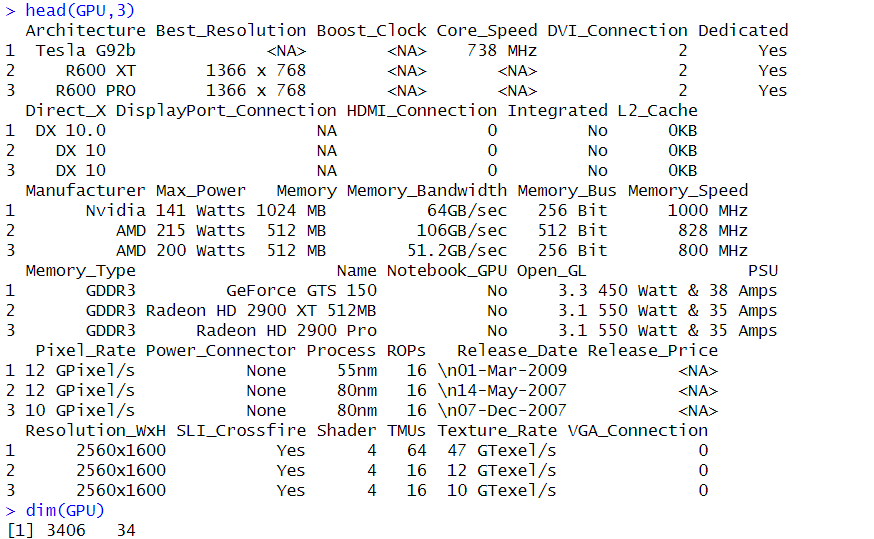
\includegraphics[width=0.75\linewidth]{images/Screenshot 2025-07-29 105142.png}}
    \caption{Các biến có trong dữ liệu ban đầu}
    \label{fig:enter-label}
\end{figure}

\textbf{Nhận xét:}
Kết quả cho thấy, bộ dữ liệu bao gồm 3406 quan sát và 34 biến, tuy nhiên lại có rất nhiều biến chứa dữ liệu khuyết dù chỉ mới xuất ra màn hình 3 dòng đầu. Chính vì thế, việc phân tích dữ liệu khuyết và chọn lọc các biến liên tục và biến phân loại phải được thực hiện một cách hợp lý, tạo tiền đề cho các phân tích chuyên sâu.

\section{Chọn biến và xử lí dữ liệu}
\textbf{a) Cơ sở lựa chọn biến}

Ta thực hiện in bảng thống kê số lượng và tỷ lệ dữ liệu khuyết trong tệp tin bằng các câu lệnh:
\begin{minted}{r}
plot1 <- ggplot(data = na_summary_df, aes(x = reorder(Variable, -Missing), y = Missing)) +
  geom_bar(stat = "identity", fill = "sienna3") +
  geom_text(aes(label = Missing), vjust = -0.5, size = 3) +
  labs(
    title = "Số lượng dữ liệu khuyết theo biến",
    x = "Biến",
    y = "Số lượng dữ liệu NA"
  ) +
  theme_minimal() +
  theme(axis.text.x = element_text(angle = 90, hjust = 1))

plot2 <- ggplot(data = na_summary_df, aes(x = reorder(Variable, -Percentage), y = Percentage)) +
  geom_bar(stat = "identity", fill = "turquoise3") +
  geom_text(aes(label = Percentage), vjust = -0.5, size = 2.5) +
  labs(
    title = "Phần trăm dữ liệu khuyết theo biến",
    x = "Biến",
    y = "Phần trăm dữ liệu NA"
  ) +
  theme_minimal() +
  theme(axis.text.x = element_text(angle = 90, hjust = 1))
plot1 | plot2
ggsave("na_combined_filtered_plot.png", width = 5, height = 12)
\end{minted}

\newpage

\textbf{Ta thu được kết quả như hình 3.2:}
\vspace{0.5cm}
\begin{figure}[!h]
    \centering
    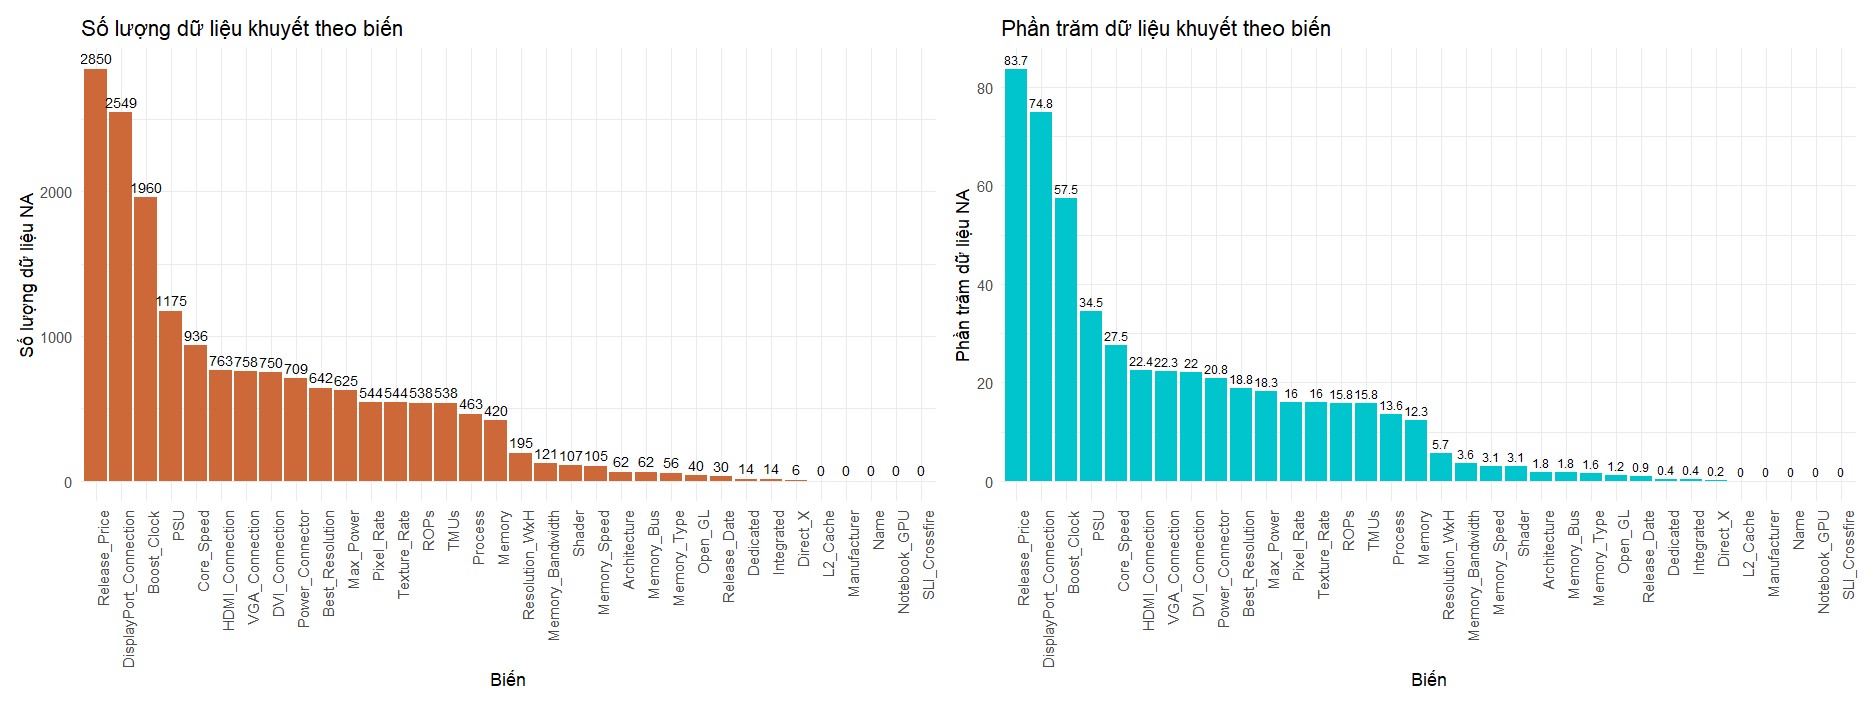
\includegraphics[width=1\linewidth]{images/Rplot01.png}
    \caption{Phân tích dữ liệu khuyết của từng biến trong bộ dữ liệu}
    \label{fig:enter-label}
\end{figure}

\textbf{Nhận xét:}
Ta nhận thấy tỷ lệ dữ liệu khuyết ở các biến có sự khác biệt và chênh lệch nhau lớn. Do đó, đối với những biến có tỷ lệ dữ liệu khuyết cao, ta sẽ không lựa chọn mà chỉ giữ lại các biến có dữ liệu khuyết tương đối.

Qua các cơ sở trên, nhằm tối ưu hóa kết quả khi phân tích hiệu năng GPU máy tính, nhóm quyết định lựa chọn các biến sau:
\colorbox{blue!10}{\hspace{2pt}\textbf{Resolution\_WxH}\hspace{2pt}},
\colorbox{blue!10}{\hspace{2pt}\textbf{Manufacturer}\hspace{2pt}},
\colorbox{blue!10}{\hspace{2pt}\textbf{Core\_Speed}\hspace{2pt}},
\colorbox{blue!10}{\hspace{2pt}\textbf{Memory\_Speed}\hspace{2pt}},
\colorbox{blue!10}{\hspace{2pt}\textbf{Memory\_Type}\hspace{2pt}},
\colorbox{blue!10}
{\hspace{2pt}\textbf{ROPs}\hspace{2pt}},
\colorbox{blue!10}{\hspace{2pt}\textbf{TMUs}\hspace{2pt}},
\colorbox{blue!10}{\hspace{2pt}\textbf{Memory\_Bus}\hspace{2pt}},
\colorbox{blue!10}{\hspace{2pt}\textbf{Memory}\hspace{2pt}},
\colorbox{blue!10}{\hspace{2pt}\textbf{Process}\hspace{2pt}},
\colorbox{blue!10}{\hspace{2pt}\textbf{Shader}\hspace{2pt}},
\colorbox{blue!10}{\hspace{2pt}\textbf{Pixel\_Rate}\hspace{2pt}} (trong đó gồm 3 biến phân loại là
\newline
\colorbox{red!10}{\hspace{2pt}\textbf{Resolution\_WxH}\hspace{2pt}},
\colorbox{red!10}{\hspace{2pt}\textbf{Manufacturer}\hspace{2pt}}, \colorbox{red!10}{\hspace{2pt}\textbf{Memory\_Type}\hspace{2pt}} và 9 biến liên tục) vì các biến này cung cấp cái nhìn toàn diện về hiệu năng GPU, từ sức mạnh xử lý, khả năng kết xuất, đến hiệu quả công nghệ, giúp nhóm đánh giá và so sánh các GPU một cách chi tiết.


% \textbf{1. Resolution\_WxH (Độ phân giải)}

% \begin{itemize}
%     \item \textbf{\textbf{Lý do chọn:}} Độ phân giải tối đa mà GPU hỗ trợ (ví dụ: 1920x1080, 4K, 8K) ảnh hưởng trực tiếp đến khả năng xử lý hình ảnh và đồ họa. GPU có khả năng hỗ trợ độ phân giải cao thường có hiệu năng tốt hơn, đặc biệt trong các ứng dụng như chơi game, chỉnh sửa video, hoặc mô phỏng 3D.
%     \item \textbf{Ý nghĩa:} Biến này giúp đánh giá khả năng hiển thị hình ảnh sắc nét và mượt mà trên các màn hình độ phân giải cao.
% \end{itemize}

% \textbf{2. Manufacturer (Nhà sản xuất)}

% \begin{itemize}
%     \item \textbf{\textbf{Lý do chọn:}} Nhà sản xuất (ví dụ: NVIDIA, AMD, Intel) ảnh hưởng đến chất lượng, độ tin cậy, công nghệ độc quyền (như CUDA của NVIDIA hoặc RDNA của AMD), và hiệu năng tối ưu hóa của GPU. Mỗi nhà sản xuất có các dòng sản phẩm với đặc điểm riêng, phù hợp với các mục đích sử dụng khác nhau (gaming, AI, thiết kế).
%     \item \textbf{Ý nghĩa:} Biến này giúp phân loại GPU theo thương hiệu và so sánh hiệu năng giữa các nhà sản xuất.
% \end{itemize}

% \textbf{3. Boost\_Clock (Tần số tăng tốc)}

% \begin{itemize}
%     \item \textbf{\textbf{Lý do chọn:}} Tần số tăng tốc (Boost Clock, tính bằng MHz hoặc GHz) là tốc độ xung nhịp tối đa mà GPU có thể đạt được khi hoạt động ở chế độ tối ưu. Tần số cao hơn thường tương ứng với hiệu năng xử lý tốt hơn, đặc biệt trong các tác vụ yêu cầu tính toán nhanh.
%     \item \textbf{Ý nghĩa:} Biến này phản ánh sức mạnh xử lý của GPU khi hoạt động ở điều kiện lý tưởng.
% \end{itemize}

% \textbf{4. Core\_Speed (Tốc độ lõi cơ bản)}

% \begin{itemize}
%     \item \textbf{\textbf{Lý do chọn:}} Tốc độ lõi cơ bản (Base Clock) là tốc độ xung nhịp mặc định của GPU. Đây là chỉ số cơ bản để đánh giá hiệu năng ban đầu, trước khi GPU tăng tốc (boost). Sự khác biệt giữa Core Speed và Boost Clock cũng cho thấy khả năng ép xung của GPU.
%     \item \textbf{Ý nghĩa:} Biến này giúp đánh giá hiệu năng cơ bản và tiềm năng tối ưu hóa của GPU.
% \end{itemize}

% \textbf{5. Memory\_Speed (Tốc độ bộ nhớ)}

% \begin{itemize}
%     \item \textbf{\textbf{Lý do chọn:}} Tốc độ bộ nhớ (thường tính bằng MHz hoặc Gbps) quyết định tốc độ truy xuất dữ liệu từ bộ nhớ GPU (VRAM). Tốc độ bộ nhớ cao giúp GPU xử lý nhanh các tác vụ đồ họa phức tạp, như kết xuất hình ảnh hoặc xử lý texture.
%     \item \textbf{Ý nghĩa:} Biến này quan trọng trong việc đánh giá khả năng xử lý dữ liệu đồ họa lớn.
% \end{itemize}

% \textbf{6. Memory\_Type (Loại bộ nhớ)}

% \begin{itemize}
%     \item \textbf{\textbf{Lý do chọn:}} Loại bộ nhớ (ví dụ: GDDR5, GDDR6, HBM2) ảnh hưởng đến băng thông và hiệu suất truyền dữ liệu của GPU. Các loại bộ nhớ mới hơn (như GDDR6X hoặc HBM3) thường cung cấp băng thông cao hơn, cải thiện hiệu năng trong các ứng dụng đồ họa nặng.
%     \item \textbf{Ý nghĩa:} Biến này giúp so sánh hiệu quả của các công nghệ bộ nhớ khác nhau.
% \end{itemize}

% \textbf{7. ROPs (Raster Operation Pipelines)}

% \begin{itemize}
%     \item \textbf{\textbf{Lý do chọn:}} ROPs là các đơn vị xử lý raster hóa, chịu trách nhiệm cho việc kết xuất pixel cuối cùng lên màn hình. Số lượng ROPs cao hơn thường cho phép GPU xử lý nhanh hơn các tác vụ liên quan đến pixel, như chống răng cưa (anti-aliasing) hoặc đổ bóng.
%     \item \textbf{Ý nghĩa:} Biến này quan trọng trong việc đánh giá hiệu năng kết xuất đồ họa.
% \end{itemize}

% \textbf{8. TMUs (Texture Mapping Units)}

% \begin{itemize}
%     \item \textbf{\textbf{Lý do chọn:}} TMUs chịu trách nhiệm ánh xạ texture lên các đối tượng 3D. Số lượng TMUs cao hơn giúp GPU xử lý texture nhanh hơn, cải thiện chất lượng và tốc độ hiển thị trong game hoặc ứng dụng 3D.
%     \item \textbf{Ý nghĩa:} Biến này ảnh hưởng đến hiệu năng trong các tác vụ liên quan đến texture.
% \end{itemize}

% \textbf{9. Memory\_Bus (Độ rộng bus bộ nhớ)}

% \begin{itemize}
%     \item \textbf{\textbf{Lý do chọn:}} Độ rộng bus bộ nhớ (tính bằng bit, ví dụ: 128-bit, 256-bit) quyết định lượng dữ liệu mà GPU có thể truyền từ bộ nhớ trong một chu kỳ. Bus rộng hơn giúp tăng băng thông, cải thiện hiệu năng khi xử lý dữ liệu lớn.
%     \item \textbf{Ý nghĩa:} Biến này quan trọng trong việc đánh giá khả năng truyền dữ liệu của GPU.
% \end{itemize}

% \textbf{10. Memory (Dung lượng bộ nhớ)}

% \begin{itemize}
%     \item \textbf{Lý do chọn:} Dung lượng bộ nhớ (VRAM, tính bằng GB) xác định lượng dữ liệu đồ họa mà GPU có thể lưu trữ. Dung lượng lớn hơn cho phép GPU xử lý các texture lớn, độ phân giải cao, hoặc nhiều tác vụ cùng lúc (như chơi game 4K hoặc học sâu).
%     \item \textbf{Ý nghĩa:} Biến này ảnh hưởng đến hiệu năng trong các ứng dụng đòi hỏi bộ nhớ lớn.
% \end{itemize}

% \textbf{11. Process (Quy trình sản xuất)}

% \begin{itemize}
%     \item \textbf{Lý do chọn:} Quy trình sản xuất (tính bằng nm, ví dụ: 7nm, 5nm) cho biết kích thước bóng bán dẫn trong chip GPU. Quy trình nhỏ hơn thường mang lại hiệu năng cao hơn, tiêu thụ ít điện hơn, và tỏa nhiệt thấp hơn.
%     \item \textbf{Ý nghĩa:} Biến này giúp đánh giá hiệu quả năng lượng và tiềm năng hiệu năng của GPU.
% \end{itemize}

% \textbf{12. Shader (Số lượng đơn vị Shader)}

% \begin{itemize}
%     \item \textbf{Lý do chọn:} Số lượng đơn vị shader (CUDA Cores của NVIDIA hoặc Stream Processors của AMD) quyết định khả năng xử lý song song của GPU. Số lượng shader cao hơn cho phép GPU thực hiện nhiều phép tính đồng thời, cải thiện hiệu năng trong các tác vụ như render 3D hoặc tính toán AI.
%     \item \textbf{Ý nghĩa:} Biến này là chỉ số quan trọng để đánh giá sức mạnh tính toán của GPU.
% \end{itemize}

% \textbf{13. Pixel\_Rate (Tốc độ điền pixel)}

% \begin{itemize}
%     \item \textbf{Lý do chọn:} Tốc độ điền pixel (Pixel Rate, tính bằng GPixel/s) đo lường khả năng GPU vẽ pixel lên màn hình mỗi giây. Pixel Rate cao hơn cho thấy GPU có khả năng xử lý nhanh các tác vụ đồ họa, đặc biệt ở độ phân giải cao.
%     \item \textbf{Ý nghĩa:} Biến này phản ánh hiệu năng kết xuất hình ảnh của GPU.
% \end{itemize}

Câu lệnh thực hiện: 
\begin{minted}{r}
GPU_new = GPU[,c("Resolution_WxH", "Manufacturer", "Core_Speed",
                 "Memory_Speed", "Memory_Type", 
                 "ROPs", "TMUs", "Memory_Bus", "Memory", 
                 "Process", "Shader", "Pixel_Rate")]
\end{minted}

\textbf{b) Xử lí dữ liệu từ các biến đã chọn}

Tiếp theo ta tạo 1 bản tóm tắt thống kê của dataframe của GPU\_new:
\begin{minted}{r}
    print(summary(GPU_new))
\end{minted}

\newpage
\textbf{Kết quả:}
\begin{figure}[!h]
    \centering
    \fbox{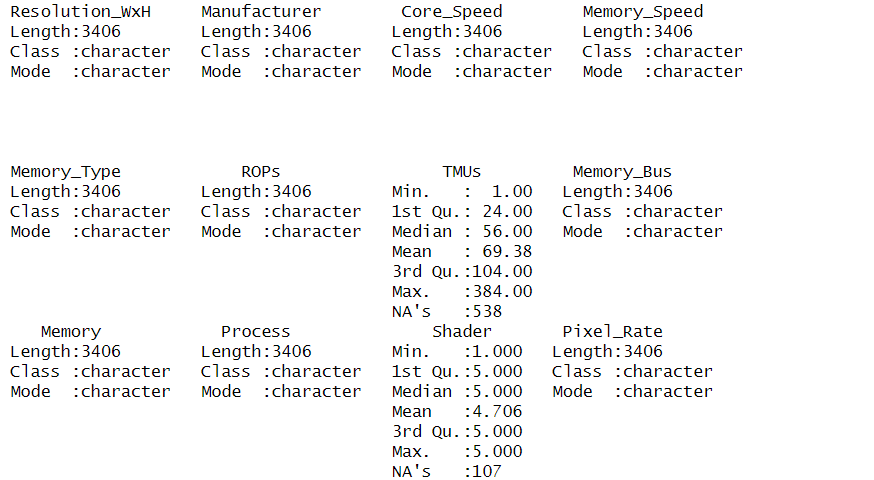
\includegraphics[width=1\linewidth]{images/Screenshot 2025-08-06 231813.png}}
    \caption{Dữ liệu từ dataframe GPU\_new}
    \label{fig:enter-label}
\end{figure}

\textbf{Nhận xét:}

\begin{itemize}
    \item \textbf{Đối với các biến định lượng:}
\end{itemize}

Hầu hết đều ở dạng character (dạng ký tự). Chính vì thế, để có thể phân tích bằng R, ta sẽ chuyển các dữ liệu cần thiết sang số thực. Ta định nghĩa một hàm để tách các đơn vị với chữ số bằng khoảng trắng và chuyển về dạng số thực:
\begin{minted}{r}
helper <- function(x){ 
    if(is.na(x)) return(NA)
    as.double(strsplit(as.character(x), " ")[[1]][1])
}
\end{minted}
Sau đó lần lượt chuyển đổi thành dữ liệu số thực, đồng thời, đối với các dữ liệu khuyết đã chuyển thành NA ban đầu của từng biến, ta thay bằng trung vị của tất cả các dữ liệu trong biến tương ứng:
\begin{minted}{r}   
# Core_Speed
GPU_new$Core_Speed <- sapply(GPU_new$Core_Speed, helper)
GPU_new$Core_Speed[is.na(GPU_new$Core_Speed)] <- median(GPU_new$Core_Speed, na.rm = TRUE)

# Memory_Speed
GPU_new$Memory_Speed <- sapply(GPU_new$Memory_Speed, helper)
GPU_new$Memory_Speed[is.na(GPU_new$Memory_Speed)] <- median(GPU_new$Memory_Speed, na.rm = TRUE)

# ROPs
# Giả sử GPU_new$ROPs đang là character, chứa các giá trị như "24 (x4)", "48 (x2)", v.v. Ta chỉ lấy phần trước dấu ngoặc
GPU_new$ROPs <- as.numeric(sub("^([0-9]+).*", "\\1", GPU_new$ROPs))
GPU_new$ROPs[is.na(GPU_new$ROPs)] <- median(GPU_new$ROPs, na.rm = TRUE)

# TMUs
GPU_new$TMUs <- as.double(GPU_new$TMUs)
GPU_new$TMUs[is.na(GPU_new$TMUs)] <- median(GPU_new$TMUs, na.rm = 
TRUE)

# Memory_Bus
GPU_new$Memory_Bus <- sapply(GPU_new$Memory_Bus, helper)
GPU_new$Memory_Bus[is.na(GPU_new$Memory_Bus)] <- median(GPU_new$Memory_Bus, na.rm = TRUE)

# Memory
GPU_new$Memory <- sapply(GPU_new$Memory, helper)
GPU_new$Memory[is.na(GPU_new$Memory)] <- median(GPU_new$Memory, na.rm = TRUE)


# Process
GPU_new$Process <- as.double(gsub("[^0-9\\.]", "", as.character(GPU_new$Process)))
GPU_new$Process[is.na(GPU_new$Process)] <- median(GPU_new$Process, na.rm = TRUE)

# Shader
GPU_new$Shader <- as.double(GPU_new$Shader)
GPU_new$Shader[is.na(GPU_new$Shader)] <- median(GPU_new$Shader, na.rm = TRUE)

# Pixel_Rate 
GPU_new$Pixel_Rate <- sapply(GPU_new$Pixel_Rate, helper) 
GPU_new$Pixel_Rate[is.na(GPU_new$Pixel_Rate)] <- median(GPU_new$Pixel_Rate, na.rm = TRUE)
\end{minted}

\begin{itemize}
    \item \textbf{Đối với các biến định tính:}
    Ta thay các giá trị khuyết NA thành mode của biến tương ứng. Đồng thời thực hiện chuyển đổi thành factor vì đây là các biến phân nhóm.

\begin{itemize}
    \item \textbf{Resolution\_WxH:}
    Vì giá trị “4096x2160” là mode (giá trị xuất hiện nhiều nhất, chiếm 39\%) nên thay thế các giá trị khuyết bằng giá trị này. Sau đó, chúng ta thực hiện gom nhóm: 4096x2160 (39\%), 2560x1600 (34\%), Other (26\%):
    \begin{minted}{r}
# Resolution_WxH
GPU_new$Resolution_WxH[is.na(GPU_new$Resolution_WxH)] = "4096x2160"
GPU_new$Resolution_WxH <- ifelse(GPU_new$Resolution_WxH == "4096x2160", 1, ifelse(GPU_new$Resolution_WxH == "2560x1600", 2, 3)) # Gom nhóm: 4096x2160 (39%), 2560x1600 (34%), Other (26%)
GPU_new$Resolution_WxH = factor(GPU_new$Resolution_WxH)
    \end{minted}
    \item \textbf{Manufacturer:} 
        \begin{minted}{r}
# Manufacturer
GPU_new$Manufacturer = factor(GPU_new$Manufacturer)
    \end{minted}
    \item  \textbf{Memory\_Type:} Ta xóa các kí tự số và khoảng trống và chỉ giữ lại các kí tự chữ nhằm phân loại tốt hơn:
    \begin{minted}{r}
# Memory_Type
GPU_new <- GPU_new[complete.cases(GPU_new$Memory_Type), ]
GPU_new$Memory_Type = gsub("[^A-Za-z]+.*","",GPU_new$Memory_Type)
GPU_new$Memory_Type = factor(GPU_new$Memory_Type)
    \end{minted}
\end{itemize}
\end{itemize}

\section{Loại bỏ trùng lặp}
Loại bỏ trùng lặp là quá trình loại bỏ các bản ghi hoặc giá trị lặp lại trong một tập dữ liệu để đảm bảo rằng mỗi hàng hoặc giá trị chỉ xuất hiện một lần. Mục đích chính là làm sạch dữ liệu, tránh sai lệch trong phân tích hoặc mô hình hóa do các bản ghi trùng lặp gây ra.

\textbf{1. Ý nghĩa của loại bỏ trùng lặp:}

Nếu một hàng hoặc giá trị xuất hiện nhiều lần (do lỗi nhập liệu, sao chép dữ liệu, v.v.), việc loại bỏ trùng lặp giúp giữ lại chỉ một phiên bản duy nhất. Ngoài ra còn cải thiện độ chính xác bởi trùng lặp có thể làm sai lệch các thống kê (như trung bình, tổng) hoặc làm tăng sai số trong mô hình. Hơn thế, còn có thể giảm kích thước tập dữ liệu, giúp xử lý nhanh hơn.

\textbf{2. Thực hiện trong R:}
Ta sẽ so sánh bộ dữ liệu trước và sau khi đã loại bỏ trùng lặp bằng câu lệnh:
\begin{minted}{r}
    str(GPU_new)
    GPU_new <- dplyr::distinct(GPU_new)
    str(GPU_new)
\end{minted}


\textbf{Kết quả:}
\begin{figure}[!h]
    \centering
    \fbox{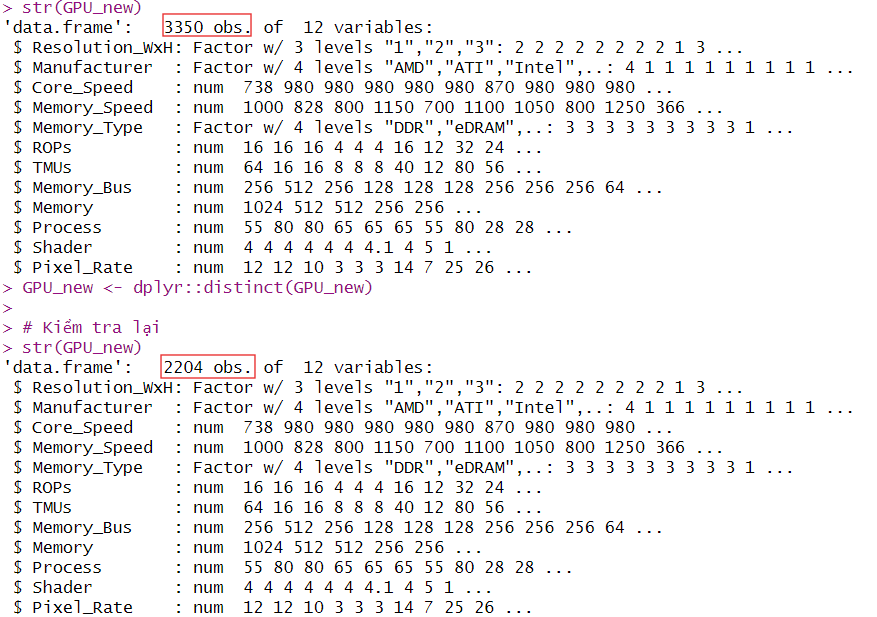
\includegraphics[width=0.9\linewidth]{images/Screenshot 2025-08-06 232835.png}}
    \caption{Hình ảnh đối chiếu trước và sau khi loại bỏ trùng lặp}
    \label{fig:enter-label}
\end{figure}

\textbf{Nhận xét:} Nhận thấy rằng trước khi loại bỏ trùng lặp, tập dữ liệu có tới 3350 quan sát, nhưng sau khi xử lý, số lượng giảm còn 2204. Điều này cho phép cải thiện đáng kể độ chính xác và tối ưu hóa dữ liệu, tạo nền tảng vững chắc để tiến hành các bước phân tích chuyên sâu tiếp theo.



% Ta tạo bảng tóm tắt các cột dữ liệu và tính tổng số giá trị thiếu (NA) trong mỗi cột
% của dataframe GPU\_new sau khi xử lý missing value:
% \begin{minted}{r}
%     print(colSums(is.na(GPU_new)))
% \end{minted}
% \begin{figure}[!h]
%     \centering
%     \fbox{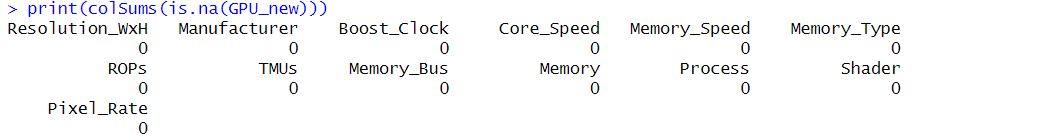
\includegraphics[width=1\linewidth]{images/Screenshot 2025-07-28 172050.png}}
% \end{figure}

% \begin{minted}{r}
%     head(GPU_new,10)
% \end{minted}
% \begin{figure}[!h]
%     \centering
%     \fbox{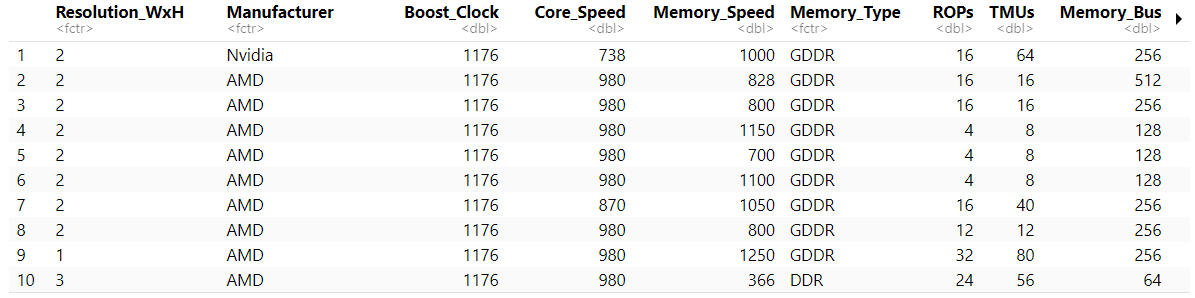
\includegraphics[width=1\linewidth]{images/Screenshot 2025-07-28 172704.png}}
% \end{figure}
% \begin{figure}[!h]
%     \centering
%     \fbox{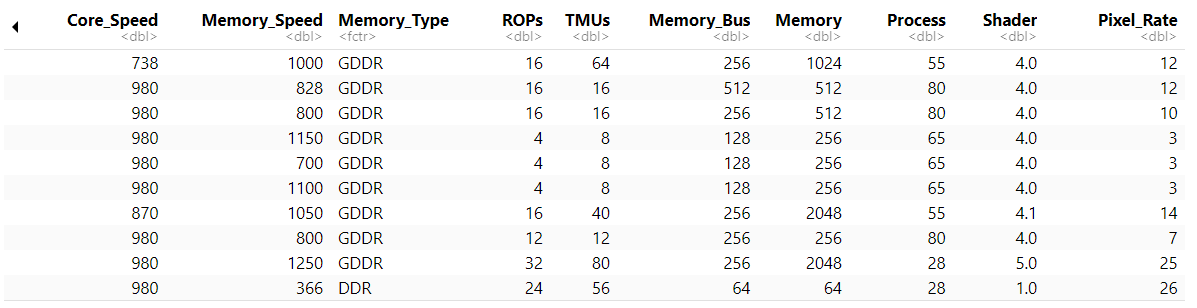
\includegraphics[width=1\linewidth]{images/Screenshot 2025-07-28 172716.png}}
% \end{figure}


% Đến thời điểm này, quá trình tiền xử lý dữ liệu đã hoàn tất thành công, khi các giá trị khuyết thiếu trong bộ dữ liệu đã được xử lý hiệu quả, đồng thời dữ liệu đã được chuẩn bị sơ bộ để sẵn sàng cho các bước thống kê tiếp theo.


\section{Chuyển đổi logarit}
Chuyển dữ liệu sang dạng log: Ta thực hiện đoạn code sau để biến đổi thành dataframe mới tên là GPU\_new\_log. 
\begin{minted}{r}
# Tạo dataframe log-transformed
GPU_new_log <- GPU_new
GPU_new_log[, numerical] <- log(GPU_new_log[, numerical])
GPU_new_log$Pixel_Rate <- log(GPU_new_log$Pixel_Rate)
\end{minted}

\textbf{*Giải thích lý do chuyển sang dạng log}
\begin{itemize}
    \item \textbf{Mối quan hệ phi tuyến tính:} Mối quan hệ giữa biến phụ thuộc và biến độc lập không tuyến tính với nhau, tức là biến độc lập ảnh hưởng đối với biến phụ thuộc không theo cách tuyến tính, mô hình hồi quy thông thường có thể không đáp ứng được. Khi mô hình hồi quy cần mô hình hóa một quan hệ phi tuyến, sử dụng logarit có thể giúp biểu diễn mối quan hệ theo cách linh hoạt và dễ dàng diễn giải.
    \item \textbf{Biến độc lập có biên độ lớn:} Khi biến độc lập có biên độ lớn và tác động không đồng nhất trên biến phụ thuộc, có thể xảy ra hiện tượng hiệu ứng không chính xác hoặc không đồng đều. Bằng cách áp dụng logarit, chúng ta giảm điều lo âu làm cho mô hình trở nên ổn định, đơn giản trong việc diễn giải và tiếp cận.
    \item \textbf{Biến phụ thuộc không tuân theo phân phối chuẩn:} Nếu biến phụ thuộc không tuân theo phân phối chuẩn, điều này có thể ảnh hưởng đến giả định của mô hình hồi quy. Áp dụng logarit có thể giúp làm cho phân phối của biến phụ thuộc gần với phân phối chuẩn hơn, từ đó cải thiện chất lượng của mô hình.
\end{itemize}
Quá trình áp dụng mô hình hồi quy với việc sử dụng logarit đòi hỏi sự cẩn trọng và chặt chẽ. Việc đưa ra quyết định này nên dựa trên quá trình kiểm tra chi tiết và sự hiểu biết sâu sắc về bản chất của dữ liệu. Điều này là chìa khóa quan trọng để đảm bảo rằng mô hình hồi quy không chỉ phản ánh chính xác mối quan hệ giữa các biến mà còn đáp ứng đúng nhu cầu và yêu cầu của vấn đề nghiên cứu.

Kiểm tra lại dữ liệu âm trong dữ liệu gốc và trong dữ liệu sau khi chuyển đổi log-transform:
\begin{minted}{r}
# Kiểm tra xem có giá trị < 0 trong dữ liệu gốc
for (var in numerical) {
    has_negative <- any(GPU_new[[var]] < 0, na.rm = TRUE)
    message(var, " in original < 0? ", has_negative)
}
\end{minted}

\begin{figure}[!h]
    \centering
    \fbox{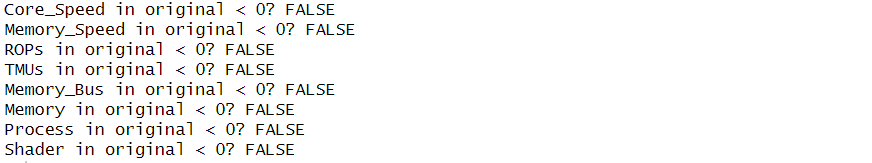
\includegraphics[width=1\linewidth]{images/Screenshot 2025-08-05 153233.png}}
\end{figure}

\begin{minted}{r}
# Kiểm tra xem có giá trị < 0 sau khi log-transform
for (var in numerical) {
 has_negative_log <- any(GPU_new_log[[var]] < 0, na.rm = TRUE)
 message(var, " in log-transformed < 0? ", has_negative_log)
}
\end{minted}

\begin{figure}[!h]
    \centering
    \fbox{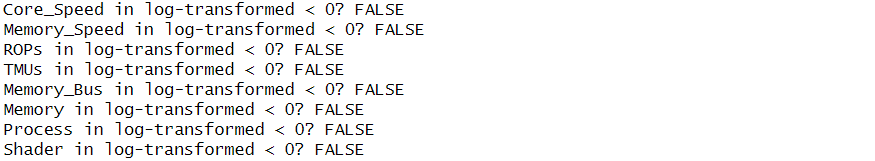
\includegraphics[width=1\linewidth]{images/Screenshot 2025-08-05 153442.png}}
\end{figure}


\section{Tổng kết}

Cuối cùng, ta tạo bảng tóm tắt các cột dữ liệu và tính tổng số giá trị thiếu (NA) trong mỗi cột của dataframe GPU\_new\_log sau khi xử lý missing value.

\begin{minted}{r}
# Thống kê nhanh trên GPU_new_log
print(summary(GPU_new_log))
print(colSums(is.na(GPU_new_log)))
\end{minted}

\begin{figure}[!h]
    \centering
    \fbox{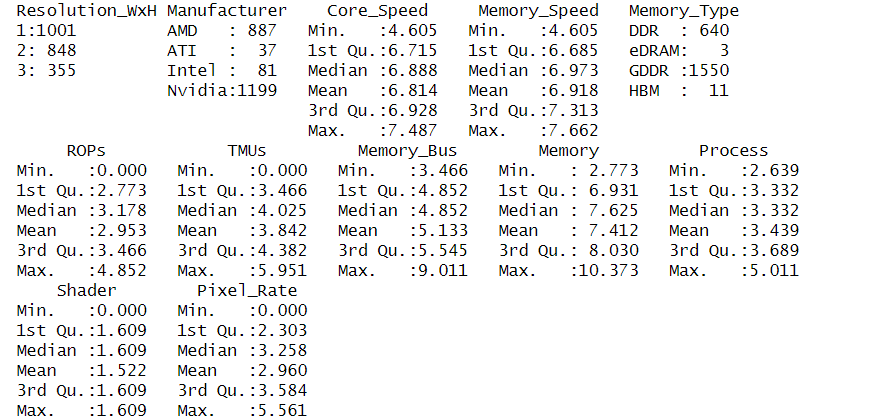
\includegraphics[width=1\linewidth]{images/Screenshot 2025-08-06 233507.png}}
\end{figure}


\begin{figure}[!h]
    \centering
    \fbox{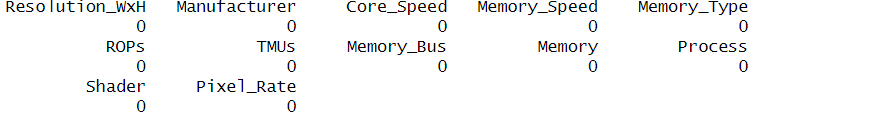
\includegraphics[width=1\linewidth]{images/Screenshot 2025-08-06 233245.png}}
\end{figure}

Đến đây xem như đã hoàn thành việc tiền xử lý số liệu bởi bộ dữ liệu đã được loại bỏ những chỗ bị khuyết cũng như đã được xử lý sơ bộ trước khi tiến hành thống kê. Sau đây, ta sẽ in ra 10 dòng đầu tiên của dataframe GPU\_new\_log. Điều này giúp ta có cái nhìn tổng quan về dữ liệu bằng cách hiển thị một phần của dataframe.

\begin{minted}{r}
# Xem 10 dòng đầu của GPU_new_log
head(GPU_new_log, 10)
\end{minted}

\begin{figure}[!h]
    \centering
    \fbox{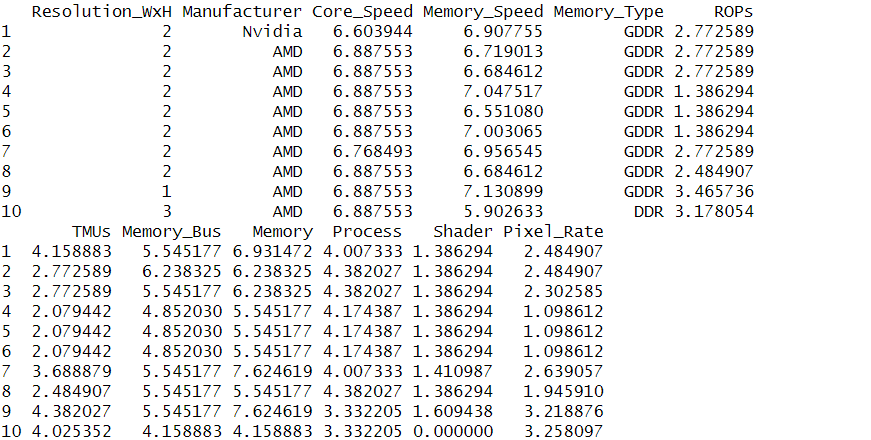
\includegraphics[width=1\linewidth]{images/Screenshot 2025-08-06 233357.png}}
\end{figure}


    \chapter{THỐNG KÊ MÔ TẢ}
    \setcounter{chapter}{4}
    \section{Thông tin tổng quát về các biến của bộ dữ liệu}

$\indent$
Sau khi làm sạch dữ liệu, ta thực hiện thống kê mô tả cho các biến đã chọn

\begin{minted}{r}
mean<-apply(GPU_new[,numerical],2,mean)
sd<-apply(GPU_new[,numerical],2,sd)
min<-apply(GPU_new[,numerical],2,min)
max<-apply(GPU_new[,numerical],2,max)
median<-apply(GPU_new[,numerical],2,median)
data.frame(mean,sd,min,max,median)
\end{minted}

\begin{figure}[!h]
    \centering
    \fbox{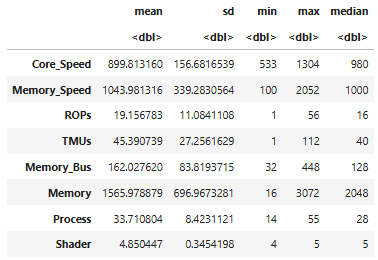
\includegraphics[width=1\linewidth]{images/Screenshot 2026-05-03 043742.png}}
\end{figure}

Tương tự, ta cũng lập bảng tính các giá trị thống kê mô tả cho các biến định lượng trong GPU\_new\_log
\begin{minted}{r}
mean<-apply(GPU_new_log[,numerical],2,mean)
sd<-apply(GPU_new_log[,numerical],2,sd)
min<-apply(GPU_new_log[,numerical],2,min)
max<-apply(GPU_new_log[,numerical],2,max)
median<-apply(GPU_new_log[,numerical],2,median)
data.frame(mean,sd,min,max,median)
\end{minted}

\begin{figure}[!h]
    \centering
    \fbox{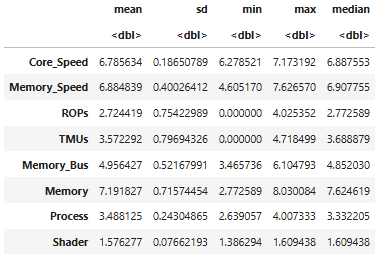
\includegraphics[width=1\linewidth]{images/Screenshot 2026-05-03 043747.png}}
\end{figure}
Để giúp chúng ta hình dung ra bản chất dữ liệu cũng như mối quan hệ giữa chúng dễ dàng hơn khi nhìn vào những con số, ta sẽ biểu diễn lại các dữ liệu này dưới dạng các biểu đồ để dễ quan sát hơn.

\section{Biểu đồ - đồ thị}
$\indent$
Biểu đồ tần suất (histogram) thường dùng để thể hiện phân phối của biến định lượng. Ta vẽ biểu đồ tần suất cho các dữ liệu GPU\_new và GPU\_new\_log. Ta tiến hành vẽ biểu đồ tần suất cho dữ liệu GPU\_new.

\begin{minted}{r}
# Chia layout thành 2 hàng và 4 cột
par(mfrow = c(2, 4), mar = c(4, 4, 2, 1))

# Vẽ histogram cho từng biến numerical trong GPU_new
for (i in 1:length(numerical)) {
 hist_data <- GPU_new[[numerical[i]]]
 hist(hist_data, 
      xlab = names(GPU_new)[which(names(GPU_new) == numerical[i])], 
      main = paste("Histogram of", names(GPU_new)[which(names(GPU_new) == numerical[i])]), 
      labels = TRUE, 
       col = "blue")
}
\end{minted}

\begin{figure}[!h]
    \centering
    \fbox{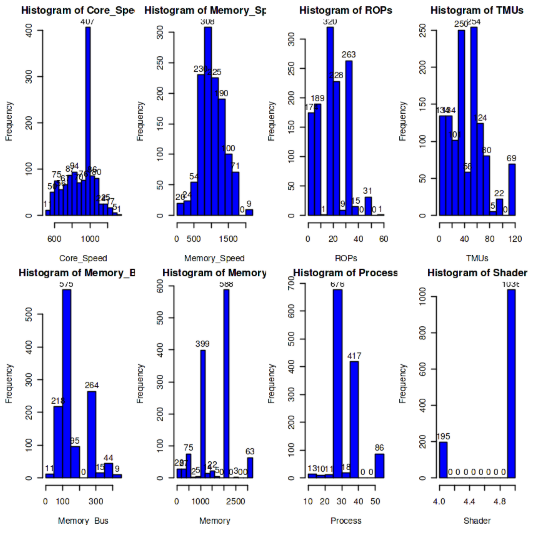
\includegraphics[width=0.8\linewidth]{images/Screenshot 2026-05-03 044605.png}}
\end{figure}

\textbf{Nhận xét:} Ta thấy các biến Process, Memory, TMUs và ROPs có phân phối lệch phải. Biến Core\_Speed có phân phối gần giống phân phối chuẩn. Trong khi đó biến Memory\_Speed có hầu hết các cột cao gần bằng nhau ngoại trừ các cột ở biên, còn biến Memory\_Bus và Shader thì gần như chỉ có một cột, các cột còn lại không đáng kể.

\vspace{0.5em}

Ta tiếp tục tiến hành vẽ biểu đồ tần suất cho dữ liệu của GPU\_new\_log.

\begin{minted}{r}
# Chia layout thành 2 hàng và 4 cột
par(mfrow = c(2, 4), mar = c(4, 4, 2, 1))

# Vẽ histogram cho từng biến numerical trong GPU_new_log
for (i in 1:length(numerical)) {
 hist_data <- GPU_new_log[[numerical[i]]]
 hist(hist_data, 
   xlab = names(GPU_new_log)[which(names(GPU_new_log) == numerical[i])], 
   main = paste("Histogram of log(", names(GPU_new_log)[which(names(GPU_new_log) == numerical[i])], ")"), 
   labels = TRUE, 
   col = "red")
}
\end{minted}

\begin{figure}[!h]
    \centering
    \fbox{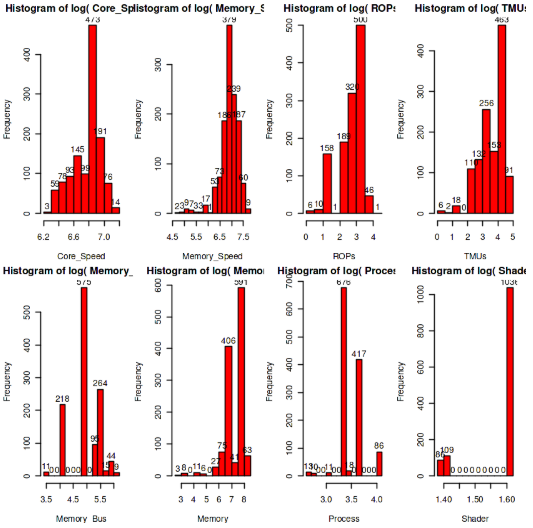
\includegraphics[width=0.8\linewidth]{images/Screenshot 2026-05-03 044612.png}}
\end{figure}

\textbf{Nhận xét:} Ta thấy sau khi chuyển đổi các biến x sang dạng log(x) thì phân phối các biến trở nên gần giống với phân phối chuẩn hơn, ví dụ như biến Memory\_Bus hay Memory\_Speed. Các biến Core\_Speed, Memory, TMUs và ROPs cũng không còn phân phối lệch như trước.

\vspace{0.5em}

Biểu đồ cột (Barplot) thường được dùng để thể hiện phân phối giữa các biến định tính. Ta tiến hành vẽ biểu đồ cột như sau:

\begin{minted}{r}
# Chia layout thành 1 hàng và 3 cột
par(mfrow = c(1, 3), mar = c(4, 4, 2, 1))

# Vẽ bảng barplot thể hiện phân phối biến định luọng
barplot(table(GPU_new$Manufacturer), xlab="Manufacturer", ylab="Frequency", main="Barplot of Manufacturer", col=c("red","green","blue"))
barplot(table(GPU_new$Memory_Type), xlab="Memory_Type", ylab="Frequency", main="Barplot of Memory_Type", col=c("red","green","blue"))
barplot(table(GPU_new$Resolution_WxH), xlab="Resolution_WxH", ylab="Frequency", main="Barplot of Resolution_WxH", col=c("red","green","blue"))
\end{minted}

\begin{figure}[!h]
    \centering
    \fbox{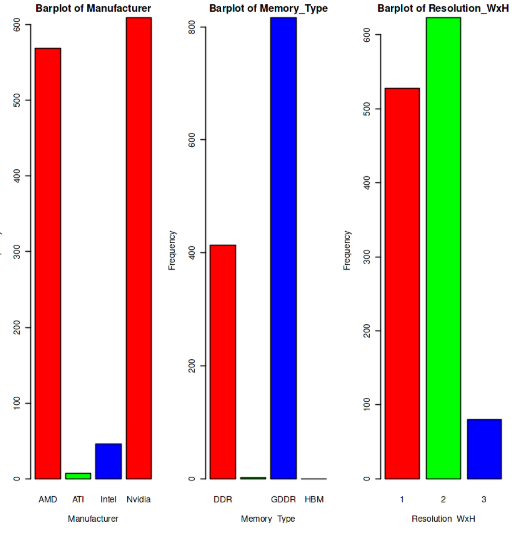
\includegraphics[width=0.8\linewidth]{images/Screenshot 2026-05-03 044739.png}}
\end{figure}

\textbf{Nhận xét:} Ta thấy hầu hết GPU đều được sản xuất bởi AMD và Nvidia, 2 nhà sản xuất còn lại (ATI và Intel) không đáng kể. Chỉ có 2 kiểu bộ nhớ là DDR và GDDR, và đa số thuộc về GDDR. Về chỉ số Resolution\_WxH thì ta thấy không có sự chênh lệch đáng kể giữa 3 cột như 2 biến kia.

\vspace{0.5em}

Biểu đồ boxplot là biểu đồ diễn tả 5 vị trí phân bố của dữ liệu: giá trị nhỏ nhất (min), tứ phân vị thứ nhất (Q1), trung vị (median), tứ phân vị thứ 3 (Q3) và giá trị lớn nhất (max). Ta vẽ biểu đồ boxplot thể hiện phân phối của biến Pixel\_Rate và log(Pixel\_Rate) theo từng phân loại của các biến rời rạc.

\begin{minted}{r}
par(mfrow=c(1,2))
boxplot(Pixel_Rate~Manufacturer, data=GPU_new, main="boxplot of Pixel_Rate for Manufacturer", col="blue")
boxplot(Pixel_Rate~Manufacturer, data=GPU_new_log, main="boxplot of log(Pixel_Rate) for Manufacturer", col="red")
\end{minted}

\begin{figure}[!h]
    \centering
    \fbox{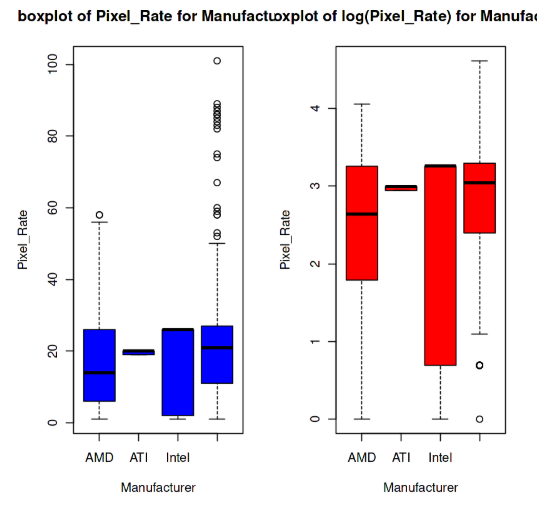
\includegraphics[width=0.6\linewidth]{images/Screenshot 2026-05-03 045147.png}}
\end{figure}

\textbf{Nhận xét:} Ta thấy với nhà sản xuất là AMD và Nvidia thì dung lượng bộ nhớ có phân phối hơi lệch phải, còn với ATI thì lệch trái. Nhưng sau khi lấy log(Pixel\_Rate) thì cả 4 phân phối đều trở thành phân phối chuẩn.

\begin{minted}{r}
par(mfrow=c(1,2))
boxplot(Pixel_Rate~Memory_Type, data=GPU_new, main="boxplot of Pixel_Rate for Memory_Type", col="blue")
boxplot(Pixel_Rate~Memory_Type, data=GPU_new_log, main="boxplot of log(Pixel_Rate) for Memory_Type", col="red")
\end{minted}

\begin{figure}[!h]
    \centering
    \fbox{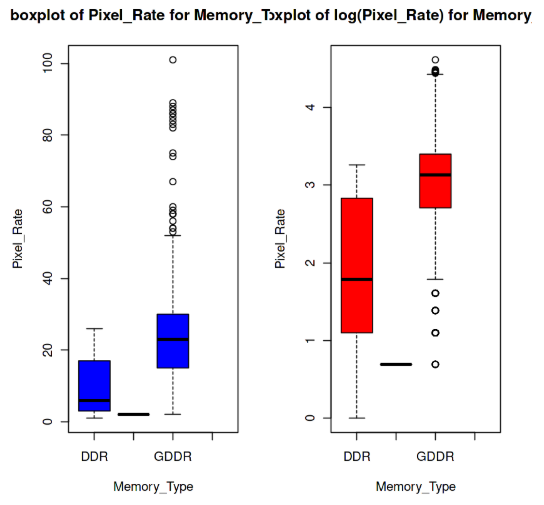
\includegraphics[width=0.6\linewidth]{images/Screenshot 2026-05-03 045152.png}}
\end{figure}

\textbf{Nhận xét:} Với kiểu bộ nhớ GDDR thì dữ liệu hơi lệch phải, còn eDRAM thì hoàn toàn lệch phải. Sau khi lấy log thì phân phối của GDDR đã trở nên phân phối chuẩn, nhưng với eDRAM thì vẫn còn bị lệch.

\begin{minted}{r}
par(mfrow=c(1,2))
boxplot(Pixel_Rate~Resolution_WxH, data=GPU_new, main="boxplot of Pixel_Rate for Resolution_WxH", col="blue")
boxplot(Pixel_Rate~Resolution_WxH, data=GPU_new_log, main="boxplot of log(Pixel_Rate) for Resolution_WxH", col="red")
\end{minted}

\begin{figure}[!h]
    \centering
    \fbox{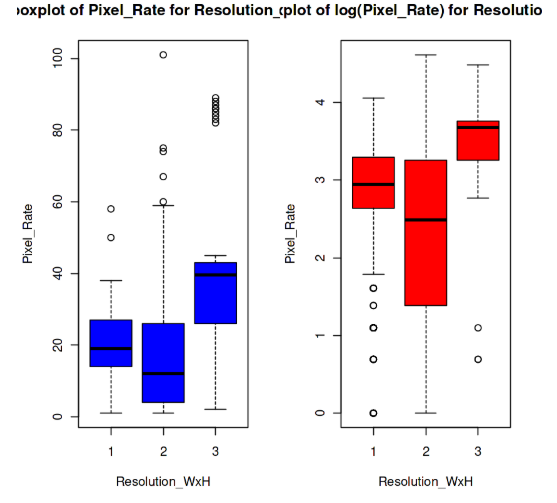
\includegraphics[width=0.6\linewidth]{images/Screenshot 2026-05-03 045158.png}}
\end{figure}

\textbf{Nhận xét:} Các phân phối ở 2 hình trên đều gần với phân phối chuẩn kể cả trước và sau khi dùng hàm log(x).

\vspace{0.5em}

Biểu đồ phân tán là biểu đồ thường được dùng để thể hiện mối liên hệ giữa 2 biến định lượng. Ta vẽ biểu đồ phân tán giữa biến Pixel\_Rate với một số biến định lượng khác.


\begin{minted}{r}
# Chia layout thành 3 hàng và 2 cột
par(mfrow = c(3, 2), mar = c(4, 4, 2, 1))
# Vẽ scatter plot
# Core_Speed vs Pixel_Rate
plot(GPU_new$Core_Speed, GPU_new$Pixel_Rate,
     xlab = "Core_Speed", ylab = "Pixel_Rate",
     main = "Pixel_Rate and Core_Speed", col = "blue", pch = 20)
fit1 <- lm(Pixel_Rate ~ Core_Speed, data = GPU_new)
abline(fit1, col = "red")
# log(Core_Speed) vs log(Pixel_Rate)
plot(GPU_new_log$Core_Speed, GPU_new_log$Pixel_Rate, 
     xlab = "log(Core_Speed)", ylab = "log(Pixel_Rate)", 
     main = "log(Pixel_Rate) and log(Core_Speed)", col = "red", pch = 20)
fit2 <- lm(Pixel_Rate ~ Core_Speed, data = GPU_new_log)
abline(fit2, col = "blue")
# ROPs vs Pixel_Rate
plot(GPU_new$ROPs, GPU_new$Pixel_Rate,
     xlab = "ROPs", ylab = "Pixel_Rate",
     main = "Pixel_Rate and ROPs", col = "blue", pch = 20)
fit3 <- lm(Pixel_Rate ~ ROPs, data = GPU_new)
abline(fit3, col = "red")
# log(ROPs) vs log(Pixel_Rate)
plot(GPU_new_log$ROPs, GPU_new_log$Pixel_Rate, 
     xlab = "log(ROPs)", ylab = "log(Pixel_Rate)", 
     main = "log(Pixel_Rate) and log(ROPs)", col = "red", pch = 20)
fit4 <- lm(Pixel_Rate ~ ROPs, data = GPU_new_log)
abline(fit4, col = "blue")
# Shader vs Pixel_Rate
plot(GPU_new$Shader, GPU_new$Pixel_Rate,
     xlab = "Shader", ylab = "Pixel_Rate",
     main = "Pixel_Rate and Shader", col = "blue", pch = 20)
fit5 <- lm(Pixel_Rate ~ Shader, data = GPU_new)
abline(fit5, col = "red")
# log(Core_Speed) vs log(Pixel_Rate)
plot(GPU_new_log$Core_Speed, GPU_new_log$Pixel_Rate, 
     xlab = "log(Shader)", ylab = "log(Pixel_Rate)", 
     main = "log(Pixel_Rate) and log(Shader)", col = "red", pch = 20)
fit6 <- lm(Pixel_Rate ~ Shader, data = GPU_new_log)
abline(fit6, col = "blue")
# Reset layout
par(mfrow = c(1, 1))
\end{minted}

\begin{figure}[!h]
    \centering
    \fbox{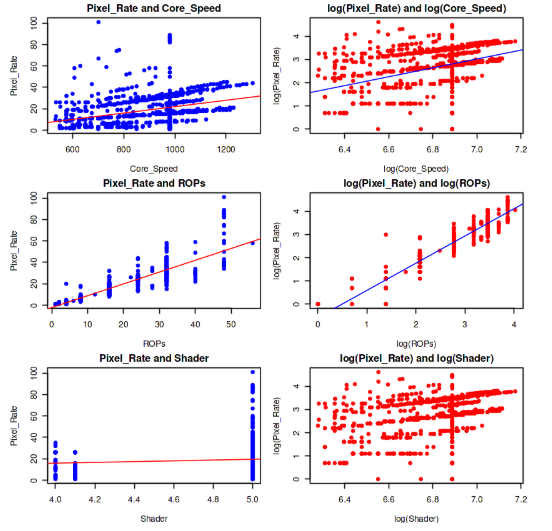
\includegraphics[width=1\linewidth]{images/Screenshot 2026-05-03 050037.png}}
\end{figure}

\textbf{Nhận xét:} Ta thấy biến Pixel\_Rate có quan hệ tuyến tính tăng với biến Core\_Speed. Điều này còn thể hiện rõ hơn giữa biến Pixel\_Rate với ROPs. Và gần như không có mối liên hệ nào giữa Pixel\_Rate và Shader.
    \chapter{THỐNG KÊ SUY DIỄN}
    \setcounter{chapter}{5}
    \section{Đánh giá mối quan hệ giữa các biến}
\subsection{Ma trận tương quan Pearson}

Ở đây ta sử dụng hệ số tương quan, là một chỉ số thống kê đo lường mối liên hệ tương quan giữa hai biến số, như Pixel\_Rate và Core\_Speed. Hệ số tương quan có giá trị từ -1 đến 1. Hệ số tương quan bằng 0 (hay gần 0) có nghĩa là hai biến số không có liên hệ gì với nhau; ngược lại nếu hệ số bằng -1 hay 1 có nghĩa là hai biến số có một mối liên hệ tuyệt đối. Nếu giá trị của hệ số tương quan là âm, có nghĩa là khi x tăng cao thì y giảm và ngược lại, khi x giảm thì y tăng. Nếu hệ số tương quan là dương, nghĩa là khi x tăng thì y cũng tăng và x giảm thì y cũng giảm.

Hệ số tương quan Pearson:

$$r = \frac{\sum_{i=1}^{n} (x_i - \bar{x})(y_i - \bar{y})}
{\sqrt{\sum_{i=1}^{n} (x_i - \bar{x})^2 \sum_{i=1}^{n} (y_i - \bar{y})^2}}
$$

Trong đó  và  là giá trị trung bình của biến số x và y.
Ta có thể kiểm định giả thiết hệ số tương quan bằng 0 (hai biến không có liên hệ) bằng hàm cor.test().

\begin{figure}[!h]
    \centering
    \fbox{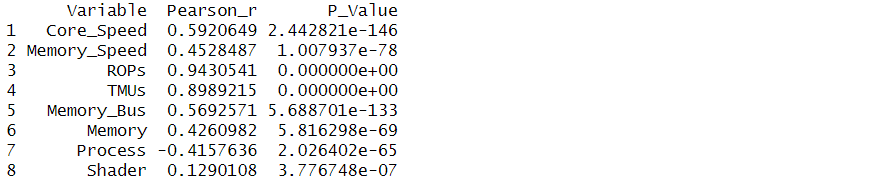
\includegraphics[width=1\linewidth]{images/Screenshot 2025-08-05 215207.png}}
\end{figure}

Như vậy, biến phụ thuộc Pixel\_Rate có quan hệ thống kê với tất cả các biến (p $<$ 0,001). Tuy nhiên với mục tiêu đơn giản hóa mô hình thì ta sẽ chọn những biến có  cao nhất là ROPs, Memory, TMUs, Core\_Speed và Memory\_Speed.

\subsection{Scatter plot và Scatter matrix}

\begin{figure}[!h]
    \centering
    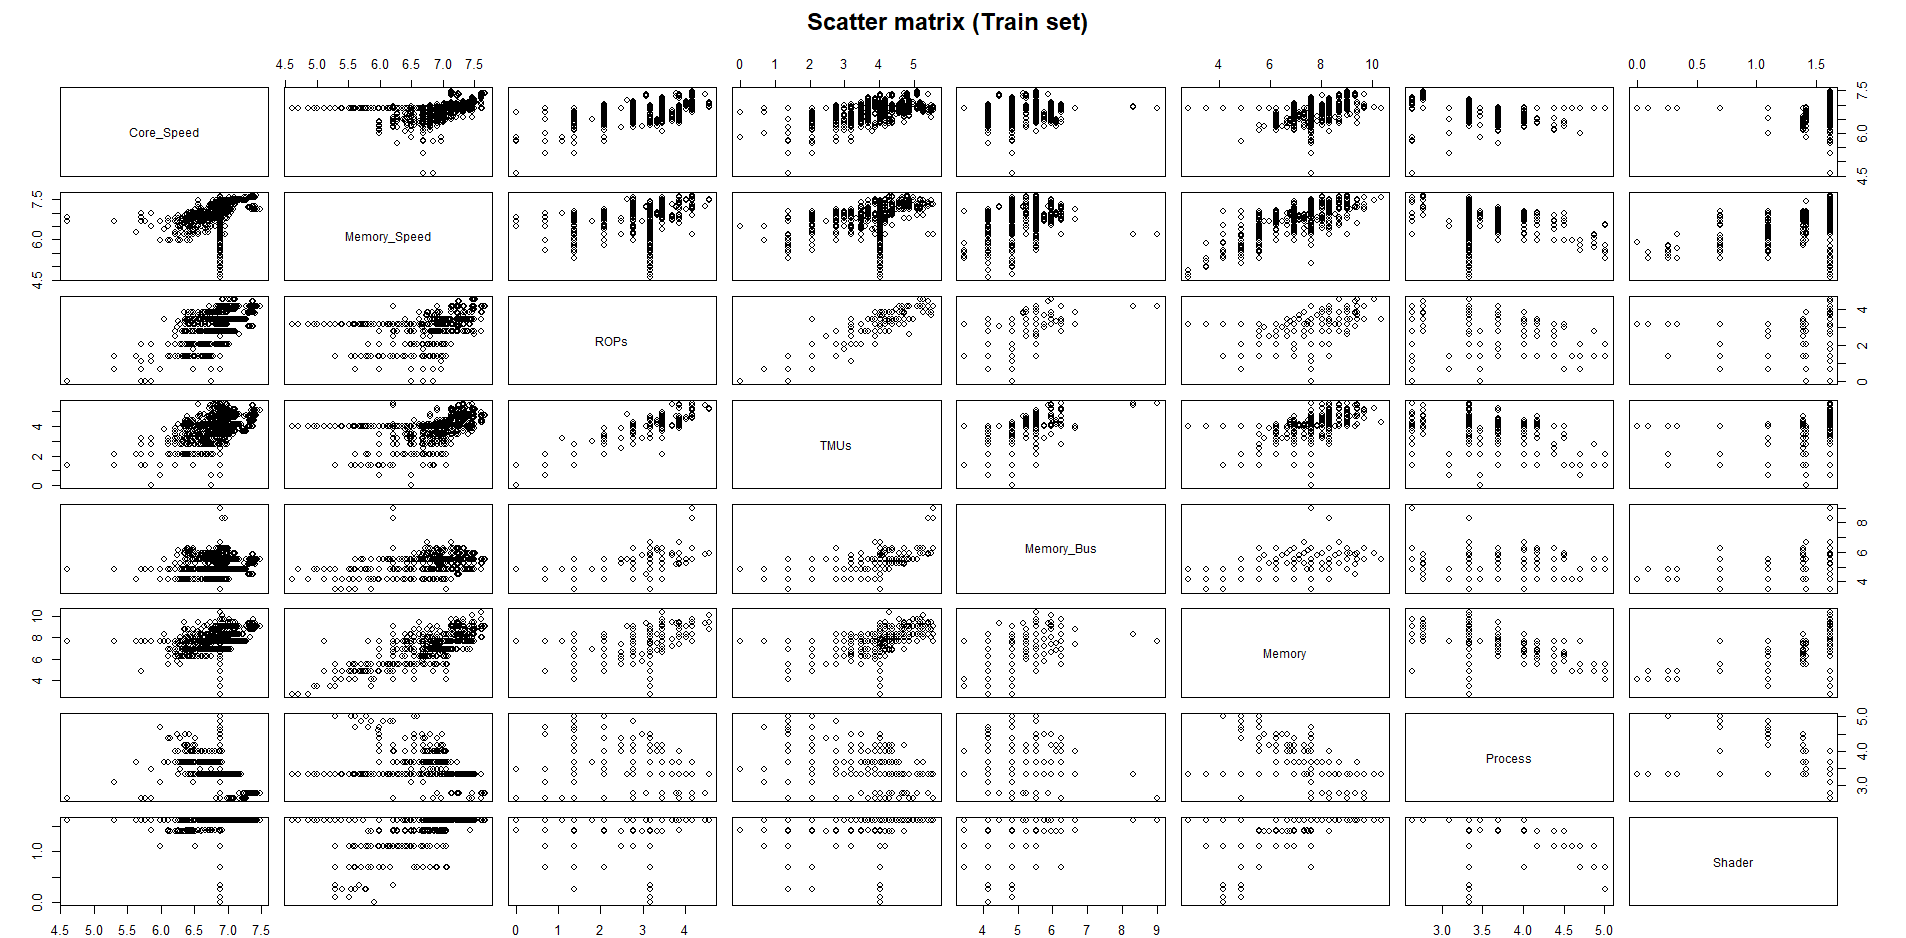
\includegraphics[width=1\linewidth]{images/Screenshot 2025-08-05 215544.png}
    \caption{Biểu đồ tương quan với hệ số tương quan giữa từng cặp biến}
\end{figure}

\section{Phân tích phương sai một yếu tố (ANOVA)}
Nhằm đánh giá sự khác biệt về hiệu suất xử lý đồ họa (Pixel\_Rate) giữa các nhóm phân loại khác nhau, Ta thực hiện phân tích phương sai (ANOVA một chiều) đối với ba biến phân loại chính Manufacturer, Memory\_Type và Resolution\_WxH trên tập huấn luyện (train).

\subsection{Mục tiêu}

\begin{itemize}
    \item Kiểm định xem liệu Pixel\_Rate có khác nhau giữa các nhóm phân loại (ví dụ Manufacturer) hay không, ở mức ý nghĩa $\alpha$ = 5%.
    \item Xác định xem có ít nhất một cặp nhóm có trung bình Pixel\_Rate khác biệt về mặt thống kê.
\end{itemize}

\subsection{Bài toán}

\subsubsection{Các điều kiện cần kiểm tra trước khi thực hiện ANOVA}

\textbf{Điều kiện 1:} Độc lập của các quan sát

Các giá trị Pixel\_Rate đo được từ mỗi nhóm (Manufacturer / Memory\_Type / Resolution\_WxH) phải được thu thập độc lập.
Kết luận: Do dữ liệu được ghi nhận từ các dòng GPU khác nhau, không có chồng lắp hay phụ thuộc, nên điều kiện này được thoả.

\textbf{Điều kiện 2:} Biến phụ thuộc là biến liên tục

Pixel\_Rate là giá trị số thực liên tục (Gpixel/s).
Kết luận: Điều kiện này được thoả.

\textbf{Điều kiện 3:} Phân phối chuẩn trong mỗi nhóm

Dùng kiểm định Shapiro–Wilk trên phần dư hoặc trực tiếp trên từng nhóm.
Nếu $p>0.05$, phần dư (hoặc dữ liệu nhóm) xấp xỉ phân phối chuẩn.

\textbf{Điều kiện 4:} Đồng nhất phương sai giữa các nhóm
Dùng Levene’s test.

Nếu $p>0.05$, không bác bỏ giả thiết phương sai bằng nhau.

\subsubsection{Giả thuyết của bài toán}
$H_0$: Trung bình Pixel\_Rate của tất cả các nhóm là bằng nhau.
$$H_0: \mu_1 = \mu_2 = \cdots = \mu_k$$

\textbf{Ví dụ với Manufacturer:}

$H_1$: Có ít nhất một cặp nhóm có trung bình Pixel\_Rate khác nhau.
$$H_A: \exists i \neq j \text{ sao cho } \mu_i \neq \mu_j
$$

Sau khi xác nhận (1) - (4), ta tiến hành ANOVA một yếu tố để kiểm định $H_0$ ở mức ý nghĩa $\alpha=0.05$. Nếu $p < 0.05$, bác bỏ $H_0$, kết luận rằng có sự khác biệt về hiệu suất Pixel\_Rate giữa các nhóm.
\subsection{Kiểm định giả thuyết}
Trước khi thực hiện phân tích phương sai (ANOVA), hai giả định quan trọng cần được kiểm tra là phân phối chuẩn trong mỗi nhóm (điều kiện 3) và đồng nhất phương sai giữa các nhóm (điều kiện 4). Các kiểm định được sử dụng bao gồm Shapiro-Wilk để đánh giá phân phối chuẩn của phần dư và Levene’s test để kiểm tra đồng nhất phương sai. Dưới đây là kết quả kiểm tra cho từng biến phân loại: Manufacturer, Memory\_Type, và Resolution\_WxH.

\subsubsection{Biến Manufacturer}
\begin{itemize}
    \item \textbf{Kiểm định Shapiro-Wilk (phân phối chuẩn của phần dư):}
    
    \textbf{\textit{Thống kê:}} W = 0.96812
    
    \textbf{\textit{Giá trị:}} $p<2.2 \times10^{-16} $
    
    \textbf{\textit{Kết luận:}} Vì p $<$ 0.05, bác bỏ giả thuyết  rằng phần dư tuân theo phân phối chuẩn. Phần dư không xấp xỉ phân phối chuẩn.
    \item \textbf{Kiểm định Levene (đồng nhất phương sai):}
    
    \textit{\textbf{Thống kê:}} F(3, 1467) = 8.799

   \textit{\textbf{Giá trị:}} $p = 8.781 \times10^{-6} $
    
   \textit{\textbf{Kết luận:}} Vì $p < 0.05$, bác bỏ giả thuyết  rằng phương sai giữa các nhóm là bằng nhau. Phương sai không đồng nhất.
\end{itemize}

\subsubsection{Biến Memory\_Type}
\begin{itemize}
    \item \textbf{Kiểm định Shapiro-Wilk (phân phối chuẩn của phần dư):}
    
    \textbf{\textit{Thống kê:}} W = 0.97858

    \textbf{\textit{Giá trị:}} $p=5.408\cdot{10}^{-14}$
    
    \textbf{\textit{Kết luận:}} Vì p $<$ 0.05, bác bỏ giả thuyết . Phần dư không tuân theo phân phối chuẩn.
    \item \textbf{Kiểm định Levene (đồng nhất phương sai):}
    
    \textbf{\textit{Thống kê:}} F(3, 1467) = 24.659
    
   \textbf{\textit{Giá trị:}} $p=1.445\cdot{10}^{-15}$
    
    \textbf{\textit{Kết luận:}} Vì p $<$ 0.05, bác bỏ giả thuyết . Phương sai giữa các nhóm không đồng nhất.
\end{itemize}

\subsubsection{Biến Resolution\_WxH}

    \begin{itemize}
        \item K\textbf{iểm định Shapiro-Wilk (phân phối chuẩn của phần dư):}
        
        \textbf{\textit{Thống kê:}} W = 0.96255
        
        \textbf{\textit{Giá trị:}} $p<2.2\cdot{10}^{-16}$
        
        \textbf{\textit{Kết luận:}} Vì p $<$ 0.05, bác bỏ giả thuyết$ H_0$. Phần dư không xấp xỉ phân phối chuẩn.
        \item \textbf{Kiểm định Levene (đồng nhất phương sai):}
        
        \textbf{\textit{Thống kê:}} F(2, 1468) = 20.193
        
        \textbf{\textit{Giá trị:}} $p=2.232\cdot{10}^{-9}$
        
        \textbf{\textit{Kết luận:}} Vì p $<$ 0.05, bác bỏ giả thuyết $H_0$. Phương sai giữa các nhóm không đồng nhất.
    \end{itemize}

\newpage
\textbf{Dựa trên phân tích, ta có kết luận:}

Kết quả từ các kiểm định Shapiro-Wilk và Levene cho thấy cả hai giả định về phân phối chuẩn và đồng nhất phương sai đều không được thỏa mãn đối với các biến Manufacturer, Memory\_Type, và Resolution\_WxH (giá trị p $<$ 0.05 trong tất cả các trường hợp). Tuy nhiên, ANOVA vẫn có thể được tiến hành nhờ tính bền vững của phương pháp này với kích thước mẫu lớn $(n \approx 1470)$, giúp giảm thiểu tác động của các vi phạm giả định.

\subsection{Tiến hành phân tích phương sai và kết quả}
Ta sử dụng hàm aov() trong R để thực hiện phân tích phương sai một yếu tố (ANOVA) cho biến Pixel\_Rate, phân loại theo các biến Manufacturer, Memory\_Type, và \ trên tập dữ liệu huấn luyện (train). Kết quả của mỗi phân tích được in ra bằng hàm summary().

Ta xây dựng mô hình:

\begin{minted}{r}
for (cat in categorical) {
  cat("\nANOVA for", cat, "on Train set\n")
  aov_mod <- aov(as.formula(paste("Pixel_Rate ~", cat)), data = train)
  print(summary(aov_mod))
}
\end{minted}

\textbf{Kết quả phân tích phương sai}

Dưới đây là kết quả ANOVA cho từng biến phân loại:

\subsubsection{Biến Manufacturer}
\begin{figure}[!h]
    \centering
    \fbox{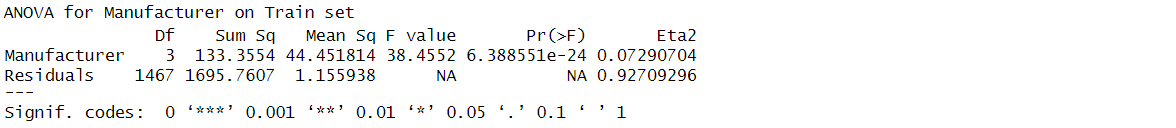
\includegraphics[width=1\linewidth]{images/Screenshot 2025-08-06 002901.png}}
\end{figure}

\textbf{Nhận xét:}

Giá trị F = 38.45 rất cao, cho thấy sự khác biệt lớn về trung bình Pixel\_Rate giữa các nhóm nhà sản xuất.

Giá trị $p < 2e-16$ (nhỏ hơn 0.05), bác bỏ giả thuyết $H_0$ rằng trung bình Pixel\_Rate của các nhà sản xuất là như nhau.

\subsubsection{Biến Memory\_Type}
\newpage
\begin{figure}[!h]
    \centering
    \fbox{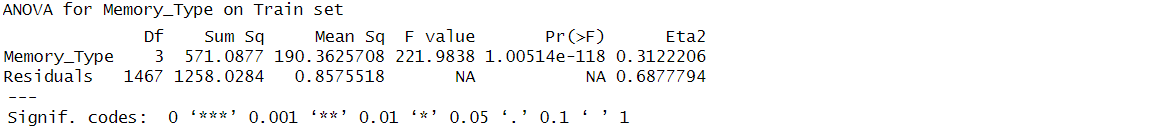
\includegraphics[width=1\linewidth]{images/Screenshot 2025-08-06 002942.png}}
\end{figure}

\textbf{Nhận xét:}

Giá trị F = 222 cực kỳ cao, cho thấy sự khác biệt đáng kể về trung bình Pixel\_Rate giữa các loại bộ nhớ.

Giá trị $p < 2e-16$, bác bỏ giả thuyết $H_0$ rằng trung bình Pixel\_Rate của các loại bộ nhớ là như nhau.

\subsubsection{Biến Resolution\_WxH}

\begin{figure}[!h]
    \centering
    \fbox{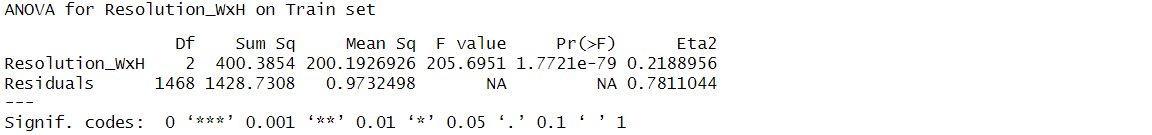
\includegraphics[width=1\linewidth]{images/Screenshot 2025-08-06 002957.png}}
\end{figure}

\textbf{Nhận xét:}

Giá trị F = 205.7 rất cao, cho thấy sự khác biệt lớn về trung bình Pixel\_Rate giữa các độ phân giải.

Giá trị$ p < 2e-16$, bác bỏ giả thuyết $H_0$ rằng trung bình Pixel\_Rate của các độ phân giải là như nhau.

\textbf{*Tổng hợp kết quả}

Dưới đây là bảng tổng hợp các giá trị đặc trưng của mô hình ANOVA cho từng biến:

\begin{longtable}{|l|c|c|c|c|}
\hline
\textbf{Biến} & \textbf{Df (giữa nhóm)} & \textbf{Df (trong nhóm)} & \textbf{Sum Sq (SSB)} & \textbf{Sum Sq (SSW)} \\
\hline
Manufacturer & 3 & 1467 & 133.4 & 1695.8 \\
\hline
Memory\_Type & 3 & 1467 & 571.1 & 1258.0 \\
\hline
Resolution\_WxH & 2 & 1468 & 400.4 & 1428.7 \\
\hline
\end{longtable}

\begin{longtable}{|l|c|c|c|c|}
\hline
\textbf{Biến}& \textbf{Mean Sq (MSB)} & \textbf{Mean Sq (MSW)} & \textbf{F value} & \textbf{p-value} \\
\hline
Manufacturer & 44.45 & 1.16 & 38.45 & $<$2e-16 \\
\hline
Memory\_Type & 190.36 & 0.86 & 222 & $<$2e-16 \\
\hline
Resolution\_WxH & 200.19 & 0.97 & 205.7 & $<$2e-16 \\
\hline
\end{longtable}

\newpage
\textbf{Ghi chú:}
\begin{itemize}
  \item \textbf{\textit{Df (giữa nhóm):}} Bậc tự do giữa các nhóm.
  \item \textbf{\textit{Df (trong nhóm):}} Bậc tự do trong nhóm (Residuals).
  \item \textbf{\textit{Sum Sq (SSB):}} Tổng bình phương giữa các nhóm.
  \item \textbf{\textit{Sum Sq (SSW):}} Tổng bình phương trong nhóm.
  \item \textbf{\textit{Mean Sq (MSB):}} Trung bình bình phương giữa các nhóm.
  \item \textbf{\textit{Mean Sq (MSW):}} Trung bình bình phương trong nhóm.
\end{itemize}

\subsection{Kết luận}

Cả ba biến đều có giá trị F rất cao: 38.45 (Manufacturer), 222 (Memory\_Type), 205.7 (Resolution\_WxH) và giá trị p $<$ 2e-16 cho cả ba biến, nhỏ hơn rất nhiều so với mức ý nghĩa thống kê $\alpha = 0.05$. Điều này cho thấy sự khác biệt rõ rệt về trung bình Pixel\_Rate giữa các nhóm theo từng biến, đồng thời ta bác bỏ giả thuyết $H_0$, kết luận rằng có sự khác biệt có ý nghĩa thống kê về Pixel\_Rate giữa các nhóm trong mỗi biến. Sự khác biệt này có thể xuất phát từ công nghệ sản xuất, chất lượng linh kiện, hoặc đặc điểm thiết kế của từng nhóm. Phân tích phương sai ANOVA cho thấy có sự khác biệt có ý nghĩa thống kê về Pixel\_Rate giữa các nhóm được chia theo biến Manufacturer, Memory\_Type, và Resolution\_WxH. Với giá trị F cao (38.45, 222, 205.7) và p-value $<$ 2e-16 cho cả ba biến. Và để làm rõ hơn về sự khác nhau này, ta sử dụng thêm câu lệnh TukeyHSD và vẽ đồ thị plot().

\subsection{Phân tích hậu nghiệm}

Để xác định cụ thể các cặp nhóm nào khác biệt đáng kể, ta tiến hành kiểm định hậu nghiệm Tukey HSD và tính toán effect size ($\eta^2$) nhằm đánh giá mức độ ảnh hưởng của từng biến đến sự biến động của Pixel\_Rate.

Ta sử dụng TukeyHSD(aov\_mod) để hậu nghiệm Tukey, tab[,"Sum Sq"] / sum(tab[ ,"Sum Sq"]) cho tính toán effect size và plot(TukeyHSD(aov\_mod), las = 1) để vẽ đồ thị:

\begin{minted}{r}
for (cat in categorical) {
  cat("\nANOVA for", cat, "on Train set\n")
  aov_mod <- aov(as.formula(paste("Pixel_Rate ~", cat)), data = train)  
  # 5.2.2 Hậu nghiệm Tukey & Effect size (η²)
  tukey_result <- TukeyHSD(aov_mod)
  print(tukey_result)
  plot(TukeyHSD(aov_mod), las = 1)
  tab <- summary(aov_mod)[[1]]
  eta2 <- tab[,"Sum Sq"] / sum(tab[,"Sum Sq"])
  print(cbind(tab, Eta2 = eta2))
}
\end{minted}

\subsubsection{Biến Manufacturer}

\textbf{Kết quả của Tukey HSD:}

\begin{figure}[!h]
    \centering
    \fbox{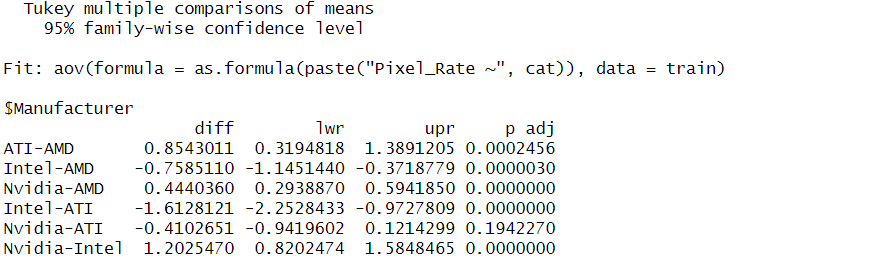
\includegraphics[width=1\linewidth]{images/Screenshot 2025-08-06 003238.png}}
\end{figure}

\textbf{Kết quả ANOVA và η²:}

\begin{figure}[!h]
    \centering
    \fbox{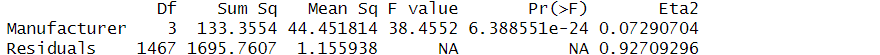
\includegraphics[width=1\linewidth]{images/Screenshot 2025-08-06 003246.png}}
\end{figure}

\textbf{Đồ thị Tukey HSD:}

\begin{figure}[!h]
    \centering
    \fbox{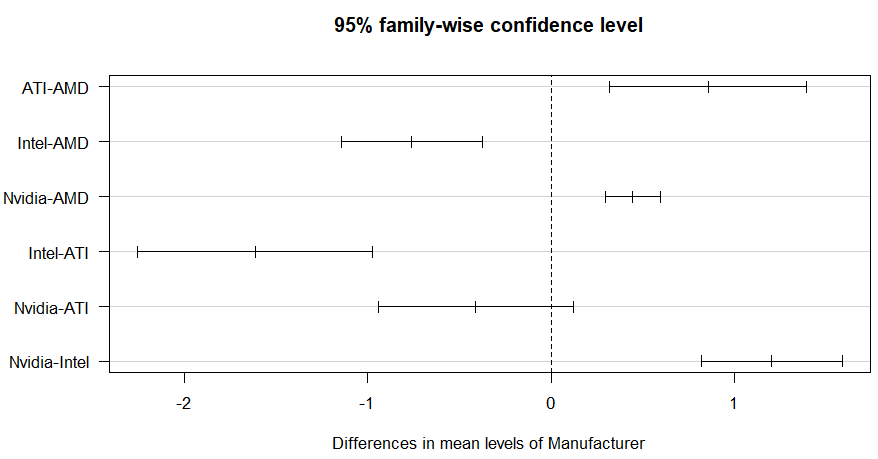
\includegraphics[width=1\linewidth]{images/Screenshot 2025-08-06 003404.png}}
\end{figure}

\newpage
\textbf{Nhận xét:}

Các cặp có $p adj < 0.05$ (có sự khác biệt đáng kể): ATI-AMD, Intel-AMD, Nvidia-AMD, Intel-ATI, và Nvidia-Intel. Riêng cặp Nvidia-ATI có p adj = 0.1942270 > 0.05, nên không có sự khác biệt đáng kể.
    \begin{itemize}
        \item \textbf{\textit{ATI-AMD:}} Giá trị diff = 0.8543011 $>$ 0, khoảng tin cậy (0.3194818, 1.3891205) không bao gồm 0, cho thấy Pixel\_Rate trung bình của ATI lớn hơn AMD $({\bar{x}}\_{ATI}$ $>$ ${\bar{x}}\_{AMD})$.
        \item \textbf{\textit{Intel-AMD:}} Giá trị diff = -0.7585110 $<$ 0, khoảng tin cậy (-1.1451440, -0.3718779) không bao gồm 0, cho thấy Pixel\_Rate trung bình của Intel nhỏ hơn AMD $({\bar{x}}\_{Intel} < {\bar{x}}\_{AMD})$.
        \item \textbf{\textit{Nvidia-AMD:}} Giá trị diff = 0.4440360 $>$ 0, khoảng tin cậy (0.2938870, 0.5941850) không bao gồm 0, cho thấy Pixel\_Rate trung bình của Nvidia lớn hơn AMD $({\bar{x}}\_{Nvidia}$ $>$ ${\bar{x}}\_{AMD})$.
        \item \textbf{\textit{Intel-ATI:}} Giá trị diff = -1.6128121 $<$ 0, khoảng tin cậy (-2.2528433, -0.9727809) không bao gồm 0, cho thấy Pixel\_Rate trung bình của Intel nhỏ hơn ATI $({\bar{x}}\_{Intel} < {\bar{x}}\_{ATI})$.
        \item \textbf{\textit{Nvidia-ATI:}} Giá trị diff = -0.4102651, khoảng tin cậy (-0.9419602, 0.1214299) bao gồm 0, phù hợp với p adj $>$ 0.05, không có sự khác biệt đáng kể.
        \item \textbf{\textit{Nvidia-Intel:}} Giá trị diff = 1.2025470 $>$ 0, khoảng tin cậy (0.8202474, 1.5848465) không bao gồm 0, cho thấy Pixel\_Rate trung bình của Nvidia lớn hơn Intel $({\bar{x}}\_{Nvidia}$ $>$ ${\bar{x}}\_{Intel})$.
    \end{itemize}
    
Từ các kết quả trên, thứ tự Pixel\_Rate trung bình là:

\begin{center}
\boxed{\textit{\textbf{ATI $>$ Nvidia $>$ AMD $>$ Intel}}}    
\end{center}
    
\textbf{Effect size (η²):} Giá trị η² = 0.0729, cho thấy biến Manufacturer giải thích khoảng 7.29\% sự biến thiên của Pixel\_Rate.

\textbf{Đồ thị Tukey HSD:} Đồ thị cho thấy các khoảng tin cậy của ATI-AMD, Intel-AMD, Nvidia-AMD, Intel-ATI, và Nvidia-Intel không giao với đường x = 0, xác nhận sự khác biệt có ý nghĩa thống kê. Riêng Nvidia-ATI có khoảng tin cậy cắt qua 0, phù hợp với kết quả không đáng kể.

\subsubsection{Biến Memory\_Type}

\textbf{Kết quả của Tukey HSD:}

\begin{figure}[!h]
    \centering
    \fbox{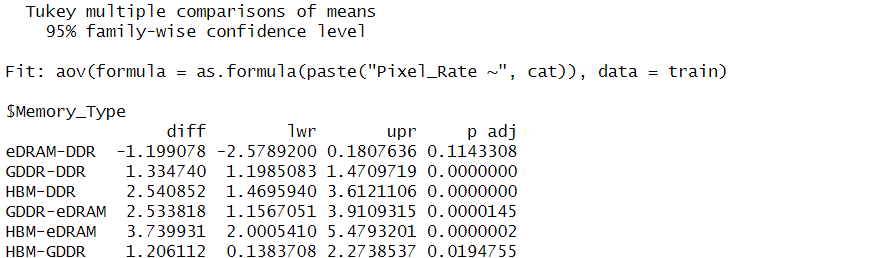
\includegraphics[width=1\linewidth]{images/Screenshot 2025-08-06 003257.png}}
\end{figure}

\textbf{Kết quả ANOVA và η²:}

\begin{figure}[!h]
    \centering
    \fbox{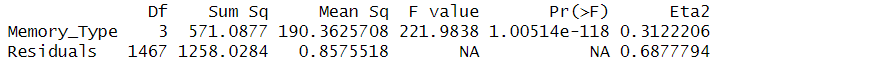
\includegraphics[width=1\linewidth]{images/Screenshot 2025-08-06 003304.png}}
\end{figure}

\textbf{Đồ thị Tukey HSD:}

\begin{figure}[!h]
    \centering
    \fbox{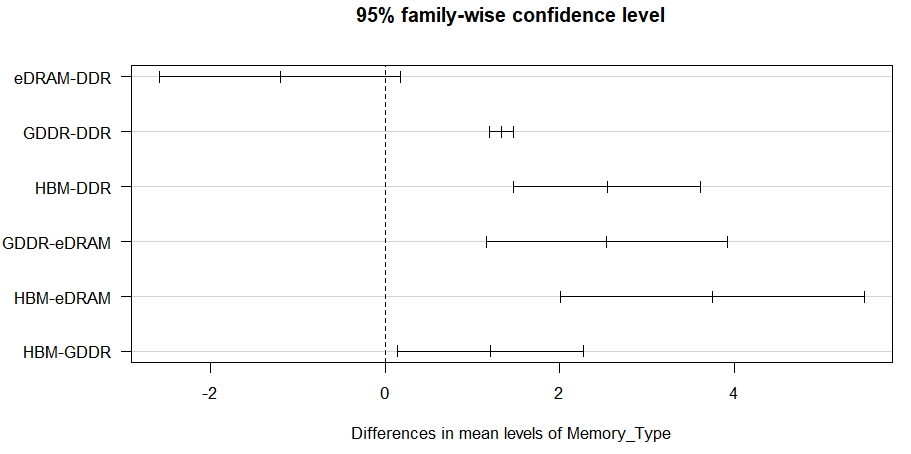
\includegraphics[width=1\linewidth]{images/Screenshot 2025-08-06 003419.png}}
\end{figure}

\textbf{Nhận xét:} Các cặp có $p adj < 0.05$ (có sự khác biệt đáng kể): \textit{GDDR-DDR, HBM-DDR, GDDR-eDRAM, HBM-eDRAM,} và \textit{HBM-GDDR}. Riêng cặp eDRAM-DDR có p adj = 0.1143308 > 0.05, không có sự khác biệt đáng kể.
    \begin{itemize}
        \item \textbf{\textit{GDDR-DDR:}} Giá trị diff$ = 1.334740 > 0$, khoảng tin cậy (1.1985083, 1.4709719) không bao gồm 0, cho thấy Pixel\_Rate trung bình của GDDR lớn hơn DDR $({\bar{x}}\_{GDDR}> {\bar{x}}\_{DDR})$.
        \item \textbf{\textit{HBM-DDR:}} Giá trị diff$ = 2.540852 > 0$, khoảng tin cậy (1.4695940, 3.6121106) không bao gồm 0, cho thấy Pixel\_Rate trung bình của HBM lớn hơn DDR $({\bar{x}}\_{HBM} > {\bar{x}}\_{DDR})$.
        \item \textbf{\textit{GDDR-eDRAM:}} Giá trịdiff  $= 2.533818 > 0$, khoảng tin cậy (1.1567051, 3.9109315) không bao gồm 0, cho thấy Pixel\_Rate trung bình của GDDR lớn hơn eDRAM $({\bar{x}}\_{GDDR} > {\bar{x}}\_{eDRAM})$.
        \item \textbf{\textit{HBM-eDRAM:}} Giá trị diff $= 3.739931 > 0$, khoảng tin cậy (2.0005410, 5.4793201) không bao gồm 0, cho thấy Pixel\_Rate trung bình của HBM lớn hơn eDRAM $({\bar{x}}\_{HBM} > {\bar{x}}\_{eDRAM})$.
        \item \textbf{\textit{HBM-GDDR:}} Giá trị diff$ = 1.206112 > 0$, khoảng tin cậy (0.1383708, 2.2738537) không bao gồm 0, cho thấy Pixel\_Rate trung bình của HBM lớn hơn GDDR $({\bar{x}}\_{HBM} > {\bar{x}}\_{GDDR})$.
    \end{itemize}
    
Từ các kết quả trên, thứ tự Pixel\_Rate trung bình là:

\begin{center}
    \boxed{\textbf{\textit{HBM $>$ GDDR $>$ DDR $>$ eDRAM}}}
\end{center}


\textbf{Effect size (η²):} Giá trị η² = 0.3122, cho thấy biến Memory\_Type giải thích khoảng 31.22\% sự biến thiên của Pixel\_Rate, mức ảnh hưởng khá lớn.

\textbf{Đồ thị Tukey HSD:} Đồ thị cho thấy các khoảng tin cậy của GDDR-DDR, HBM-DDR, GDDR-eDRAM, HBM-eDRAM, và HBM-GDDR không giao với đường x = 0, xác nhận sự khác biệt có ý nghĩa thống kê. Riêng eDRAM-DDR có khoảng tin cậy cắt qua 0, phù hợp với kết quả không đáng kể.

\subsubsection{Biến Resolution\_WxH}

\textbf{Kết quả của Tukey HSD:}

\begin{figure}[!h]
    \centering
    \fbox{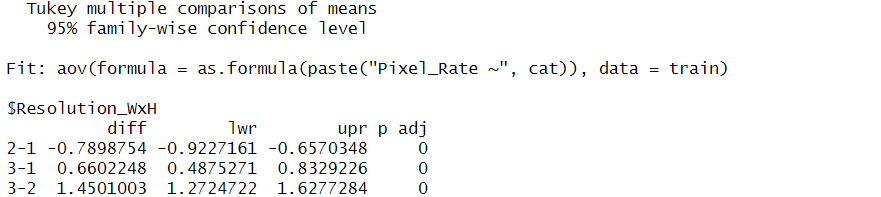
\includegraphics[width=1\linewidth]{images/Screenshot 2025-08-06 003315.png}}
\end{figure}

\newpage

\textbf{Kết quả ANOVA và η²:}

\begin{figure}[!h]
    \centering
    \fbox{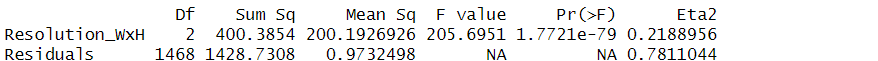
\includegraphics[width=1\linewidth]{images/Screenshot 2025-08-06 003323.png}}
\end{figure}

\textbf{Đồ thị Tukey HSD:}

\begin{figure}[!h]
    \centering
    \fbox{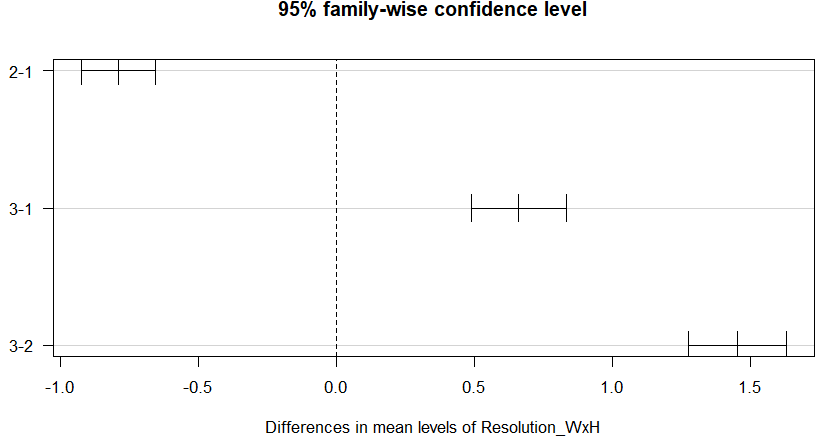
\includegraphics[width=1\linewidth]{images/Screenshot 2025-08-06 003429.png}}
\end{figure}

\textbf{Nhận xét:}

Tất cả các cặp đều có $p adj = 0 < 0.05$, cho thấy có sự khác biệt đáng kể giữa các nhóm.
    \begin{itemize}
        \item \textbf{\textit{2-1:}} Giá trị diff $= -0.7898754 < 0$, khoảng tin cậy (-0.9227161, -0.6570348) không bao gồm 0, cho thấy Pixel\_Rate trung bình của nhóm 2 nhỏ hơn nhóm 1 $({\bar{x}}\_2< {\bar{x}}\_1)$.
        \item \textbf{\textit{3-1:}} Giá trị diff $= 0.6602248 > 0$, khoảng tin cậy (0.4875271, 0.8329226) không bao gồm 0, cho thấy Pixel\_Rate trung bình của nhóm 3 lớn hơn nhóm 1 $({\bar{x}}\_3 > {\bar{x}}\_1)$.
        \item \textbf{\textit{3-2:}} Giá trị diff $= 1.4501003 > 0$, khoảng tin cậy (1.2724722, 1.6277284) không bao gồm 0, cho thấy Pixel\_Rate trung bình của nhóm 3 lớn hơn nhóm 2 $({\bar{x}}\_3 > {\bar{x}}\_2)$.
    \end{itemize}
    
Từ các kết quả trên, thứ tự Pixel\_Rate trung bình là:
\begin{center}
    \boxed{\textbf{\textit{Resolution 3 $>$ Resolution 1 $>$ Resolution 2}}}
\end{center}

\textbf{Effect size (η²):} Giá trị η² = 0.2189, cho thấy biến Resolution\_WxH giải thích khoảng 21.89\% sự biến thiên của Pixel\_Rate, mức ảnh hưởng đáng kể.

\textbf{Đồ thị Tukey HSD:} Đồ thị cho thấy tất cả các khoảng tin cậy của 2-1, 3-1, và 3-2 không giao với đường x = 0, xác nhận sự khác biệt có ý nghĩa thống kê giữa các nhóm.

\subsubsection{Kết luận}

Kết quả kiểm định hậu nghiệm Tukey HSD và effect size η² cho thấy:
\begin{itemize}
    \item \textbf{Manufacturer:} Có sự khác biệt đáng kể giữa các nhà sản xuất, với ATI có Pixel\_Rate trung bình cao nhất, nhưng η² = 0.0729 cho thấy biến này chỉ giải thích một phần nhỏ (7.29\%) sự biến thiên của Pixel\_Rate.
    \item \textbf{Memory\_Type:} Có sự khác biệt lớn giữa các loại bộ nhớ, với HBM có Pixel\_Rate trung bình cao nhất, và η² = 0.3122 cho thấy biến này có ảnh hưởng mạnh (31.22\%) đến Pixel\_Rate.
    \item \textbf{Resolution\_WxH:} Có sự khác biệt đáng kể giữa các nhóm độ phân giải, với nhóm 3 có Pixel\_Rate trung bình cao nhất, và η² = 0.2189 cho thấy biến này có ảnh hưởng đáng kể (21.89\%) đến Pixel\_Rate.
\end{itemize}
    
Kết quả này có thể được sử dụng để đánh giá tác động của các yếu tố phân loại lên hiệu suất GPU (Pixel\_Rate), từ đó hỗ trợ trong việc xây dựng mô hình hồi quy tuyến tính dự báo về sự phát triển của GPU trong mảng hiệu suất dựng ảnh.

\section{Xây dựng mô hình hồi quy đa biến}

Vấn đề đặt ra là tìm hiểu những yếu tố ảnh hưởng đến hiệu suất dựng ảnh Pixel\_Rate của GPU. Ta sẽ xây dựng mô hình hồi quy tuyến tính đa biến để giải quyết vấn đề này.
    
Mô hình hồi quy đa biến có dạng:
$$Y = \beta_0 + \beta_1 X_1 + \beta_2 X_2 + \cdots + \beta_n X_n + \epsilon$$

Đầu tiên, ta thực hiện chia tập dữ liệu thành tập train và test với tỉ lệ 2:1 và xây dựng mô hình hồi quy tuyến tính, lưu kết quả vào biến model:

\begin{minted}{r}
# Chia dữ liệu thành tập huấn luyện và tập kiểm tra (2/3 - 1/3)
set.seed(123)
index <- createDataPartition(GPU_new_log$Pixel_Rate, p = 2/3, list = FALSE)
train <- GPU_new_log[index, ]
test  <- GPU_new_log[-index, ]
\end{minted}

\subsection{Kiểm tra lại các biến}
Trước khi xây dựng mô hình hồi quy tuyến tính đa biến để dự đoán Pixel\_Rate, ta tiến hành các bước kiểm tra dữ liệu và lựa chọn biến nhằm đảm bảo mô hình đạt độ chính xác cao, tránh hiện tượng đa cộng tuyến và tối ưu hóa hiệu suất. Quá trình này bao gồm kiểm tra đa cộng tuyến bằng VIF, lựa chọn biến bằng phương pháp stepwise selection, và áp dụng feature engineering (đã làm ở trên bước xử lí dữ liệu và thống kê mô tả) để cải thiện chất lượng dữ liệu.

\subsubsection{Kiểm tra đa cộng tuyến bằng VIF}
Ta bắt đầu bằng cách xây dựng một mô hình hồi quy đầy đủ bao gồm tất cả các biến định lượng (Core\_Speed, Memory\_Speed, ROPs, TMUs, Memory\_Bus, Memory, Process, Shader) và biến phân loại (Manufacturer, Memory\_Type, Resolution\_WxH). Hệ số VIF (Variance Inflation Factor) được tính toán để kiểm tra hiện tượng đa cộng tuyến giữa các biến, sử dụng đoạn mã sau:

\begin{minted}{r}
# Tạo công thức với tất cả biến
full_form <- as.formula(
  paste("Pixel_Rate ~", paste(c(numerical, categorical), collapse = " + "))
)
# Huấn luyện mô hình đầy đủ
full_mod <- lm(full_form, data = train)
print(vif(full_mod))  # Kiểm tra multicollinearity
\end{minted}

Kết quả thu được sau khi ta chạy đoạn mã:
\begin{figure}[!h]
    \centering
    \fbox{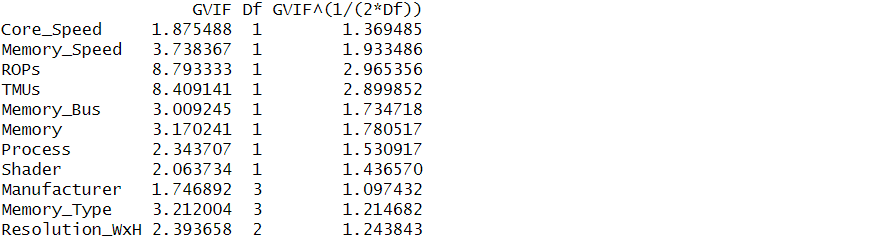
\includegraphics[width=1\linewidth]{images/Screenshot 2025-08-06 010408.png}}
\end{figure}

Các biến có VIF $<$ 5 thường được coi là không có đa cộng tuyến nghiêm trọng. Tuy nhiên, hai biến ROPs (VIF = 8.79) và TMUs (VIF = 8.41) có giá trị VIF cao, cho thấy tồn tại đa cộng tuyến giữa các biến này. Điều này có thể ảnh hưởng đến độ tin cậy của các hệ số hồi quy, do đó cần xem xét thêm trong quá trình lựa chọn biến.

\subsubsection{Lựa chọn biến bằng stepwise selection}

Để tối ưu hóa mô hình, ta sử dụng phương pháp stepwise selection (hướng "both") nhằm tự động lựa chọn các biến có ý nghĩa thống kê và loại bỏ các biến không cần thiết. Phương pháp này cải thiện độ chính xác và đơn giản hóa mô hình. Đoạn mã được sử dụng:

\begin{minted}{r}
# Lựa chọn biến bằng stepwise selection
step_mod <- step(full_mod, direction = "both", trace = 0)
print(summary(step_mod))
\end{minted}

Kết quả mô hình sau khi áp dụng stepwise selection:

\begin{figure}[!h]
    \centering
    \fbox{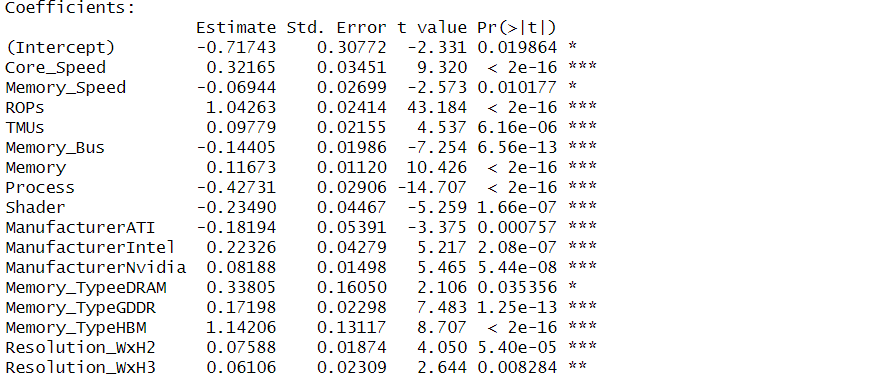
\includegraphics[width=1\linewidth]{images/Screenshot 2025-08-06 010632.png}}
\end{figure}

Sau khi áp dụng stepwise selection, mô hình vẫn giữ lại tất cả các biến ban đầu, điều này cho thấy các biến đều có ý nghĩa thống kê (p-value $<$ 0.05) trong việc dự đoán Pixel\_Rate. Tất cả các biến ban đầu đều được giữ lại, với các hệ số hồi quy có ý nghĩa thống kê cao, cho thấy chúng đóng vai trò quan trọng trong việc giải thích Pixel\_Rate.

\subsection{Xây dựng mô hình đa biến}

Ta xây dựng mô hình hồi quy tuyến tính đa biến để dự đoán Pixel\_Rate dựa trên các biến độc lập bao gồm các biến định lượng (Core\_Speed, Memory\_Speed, ROPs, TMUs, Memory\_Bus, Memory, Process, Shader) và các biến phân loại (Manufacturer, Memory\_Type, Resolution\_WxH). Mô hình được huấn luyện trên tập dữ liệu train, và kết quả được phân tích thông qua hàm summary(model\_final):

\begin{minted}{r}
# 5.3.2 Xây dựng mô hình đa biến
model_final <- step_mod
print(summary(model_final))
\end{minted}

\begin{figure}[!h]
    \centering
    \fbox{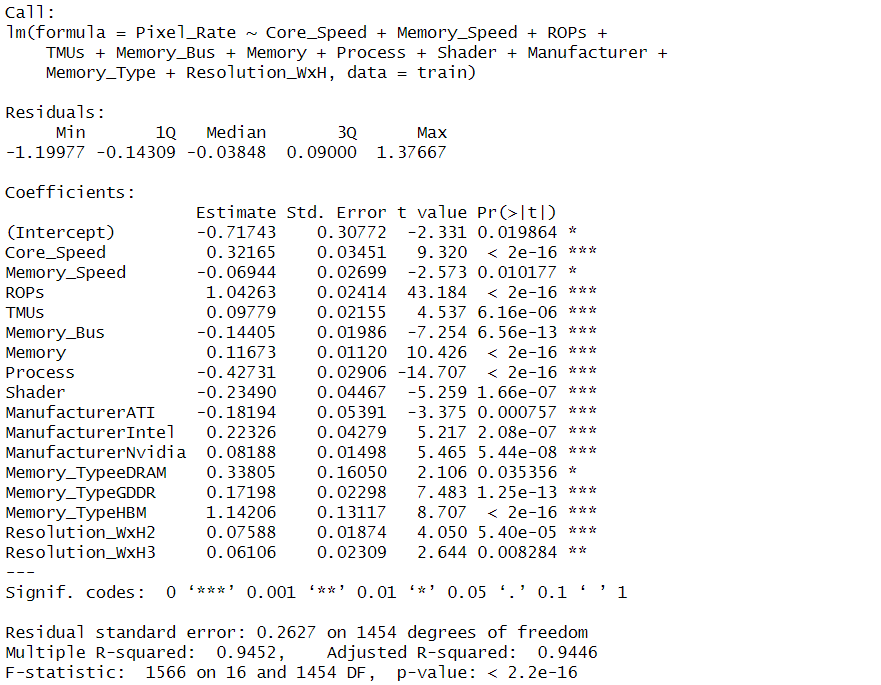
\includegraphics[width=0.75\linewidth]{images/Screenshot 2025-08-06 010852.png}}
\end{figure}

\textbf{Nhận xét:}

\begin{itemize}
    \item \textbf{Hệ số hồi quy:}
    \begin{itemize}
    \item \textbf{\textit{Intercept:}} Hệ số chặn của mô hình là -0.71743, cho biết giá trị kỳ vọng của Pixel\_Rate khi tất cả các biến dự báo bằng 0. Tuy nhiên, giá trị này có thể không mang ý nghĩa thực tiễn trong bối cảnh thực tế.
    \item \textbf{\textit{Core\_Speed:}} Hệ số hồi quy là 0.32165, cho biết khi Core\_Speed tăng thêm một đơn vị (giả sử các biến khác không thay đổi), Pixel\_Rate tăng trung bình 0.32165 đơn vị.
    \item \textbf{\textit{Memory\_Speed:}} Hệ số hồi quy là -0.06944, cho thấy khi Memory\_Speed tăng thêm một đơn vị, Pixel\_Rate giảm trung bình 0.06944 đơn vị.
    \item \textbf{\textit{ROPs:}} Hệ số hồi quy là 1.04263, cho thấy khi ROPs tăng thêm một đơn vị, Pixel\_Rate tăng trung bình 1.04263 đơn vị, thể hiện ảnh hưởng mạnh mẽ của biến này.
    \item \textbf{\textit{TMUs:}} Hệ số hồi quy là 0.09779, cho biết khi TMUs tăng thêm một đơn vị, Pixel\_Rate tăng trung bình 0.09779 đơn vị.
    \item \textbf{\textit{Memory\_Bus:}} Hệ số hồi quy là -0.14405, cho thấy khi Memory\_Bus tăng thêm một đơn vị, Pixel\_Rate giảm trung bình 0.14405 đơn vị.
    \item \textbf{\textit{Memory:}} Hệ số hồi quy là 0.11673, nghĩa là khi Memory tăng thêm một đơn vị, Pixel\_Rate tăng trung bình 0.11673 đơn vị.
    \item \textbf{\textit{Process:}} Hệ số hồi quy là -0.42731, cho biết khi Process tăng thêm một đơn vị, Pixel\_Rate giảm trung bình 0.42731 đơn vị.
    \item \textbf{\textit{Shader:}} Hệ số hồi quy là -0.23490, cho thấy khi Shader tăng thêm một đơn vị, Pixel\_Rate giảm trung bình 0.23490 đơn vị.
    \item \textbf{\textit{Manufacturer:}}
    \begin{itemize}
    \item \textbf{\textit{ManufacturerATI:}} Hệ số -0.18194, cho thấy Pixel\_Rate của ATI thấp hơn nhóm cơ sở.
    \item \textbf{\textit{ManufacturerIntel:}} Hệ số 0.22326, cho thấy Pixel\_Rate của Intel cao hơn nhóm cơ sở.
    \item \textbf{\textit{ManufacturerNvidia:}} Hệ số 0.08188, cho thấy Pixel\_Rate của Nvidia cao hơn nhóm cơ sở.
\end{itemize}
    \item \textbf{\textit{Memory\_Type:}}
\begin{itemize}
    \item \textbf{\textit{Memory\_TypeeDRAM:}} Hệ số 0.33805, cho thấy Pixel\_Rate của eDRAM cao hơn nhóm cơ sở.
    \item \textbf{\textit{Memory\_TypeGDDR:}} Hệ số 0.17198, cho thấy Pixel\_Rate của GDDR cao hơn nhóm cơ sở.
    \item \textbf{\textit{Memory\_TypeHBM:}} Hệ số 1.14206, cho thấy Pixel\_Rate của HBM cao hơn đáng kể so với nhóm cơ sở.
\end{itemize}
\item \textbf{\textit{Resolution\_WxH:}}
\begin{itemize}
    \item \textbf{\textit{Resolution\_WxH2:}} Hệ số 0.07588, cho thấy Pixel\_Rate của nhóm 2 cao hơn nhóm cơ sở.
    \item \textbf{\textit{Resolution\_WxH3:}} Hệ số 0.06106, cho thấy Pixel\_Rate của nhóm 3 cao hơn nhóm cơ sở.
\end{itemize}
\end{itemize}
\item \textbf{Ý nghĩa thống kê:}

Các giá trị p-value của tất cả các biến độc lập đều nhỏ hơn 0.05, cho thấy các biến này có ảnh hưởng ý nghĩa thống kê đến Pixel\_Rate ở mức ý nghĩa 5\%. Đặc biệt, các biến như ROPs, Process, Memory, và Core\_Speed có p-value $<$ 2e-16, thể hiện mức độ ý nghĩa thống kê rất cao.
\item \textbf{Độ phù hợp của mô hình:}
\begin{itemize}
    \item \textbf{\textit{Multiple R-squared:}} Giá trị ( $R^2$ = 0.9452 ), chỉ ra rằng khoảng 94.52\% phương sai của Pixel\_Rate được giải thích bởi mô hình hồi quy này. Đây là mức độ giải thích rất cao, cho thấy mô hình phù hợp tốt với dữ liệu.
    \item \textbf{\textit{Adjusted R-squared:}} Giá trị ( $R^2$ ) điều chỉnh là 0.9446, gần với ( $R^2$ ), cho thấy mô hình không bị overfitting dù có nhiều biến độc lập.
    \item \textbf{\textit{F-statistic:}} Giá trị F = 1566 với p-value $<$ 2.2e-16, xác nhận mô hình có ý nghĩa thống kê tổng thể.
\end{itemize}

\item \textbf{Phần dư (Residuals)}

Phần dư dao động từ -1.19977 đến 1.37667, với độ lệch chuẩn là 0.2627. Giá trị phần dư tương đối nhỏ, cho thấy mô hình dự đoán khá chính xác. Tuy nhiên, phần dư tối đa (1.37667) có thể chỉ ra rằng một số điểm dữ liệu chưa được giải thích hoàn toàn, có thể do thiếu các biến quan trọng khác.
\end{itemize}

\subsection{Đồ thị chuẩn đoán (Diagnostic plots)}

Sử dụng câu lệnh plot(model\_final) ta được 4 đồ thị như sau:

\begin{figure}[!h]
    \centering\fbox{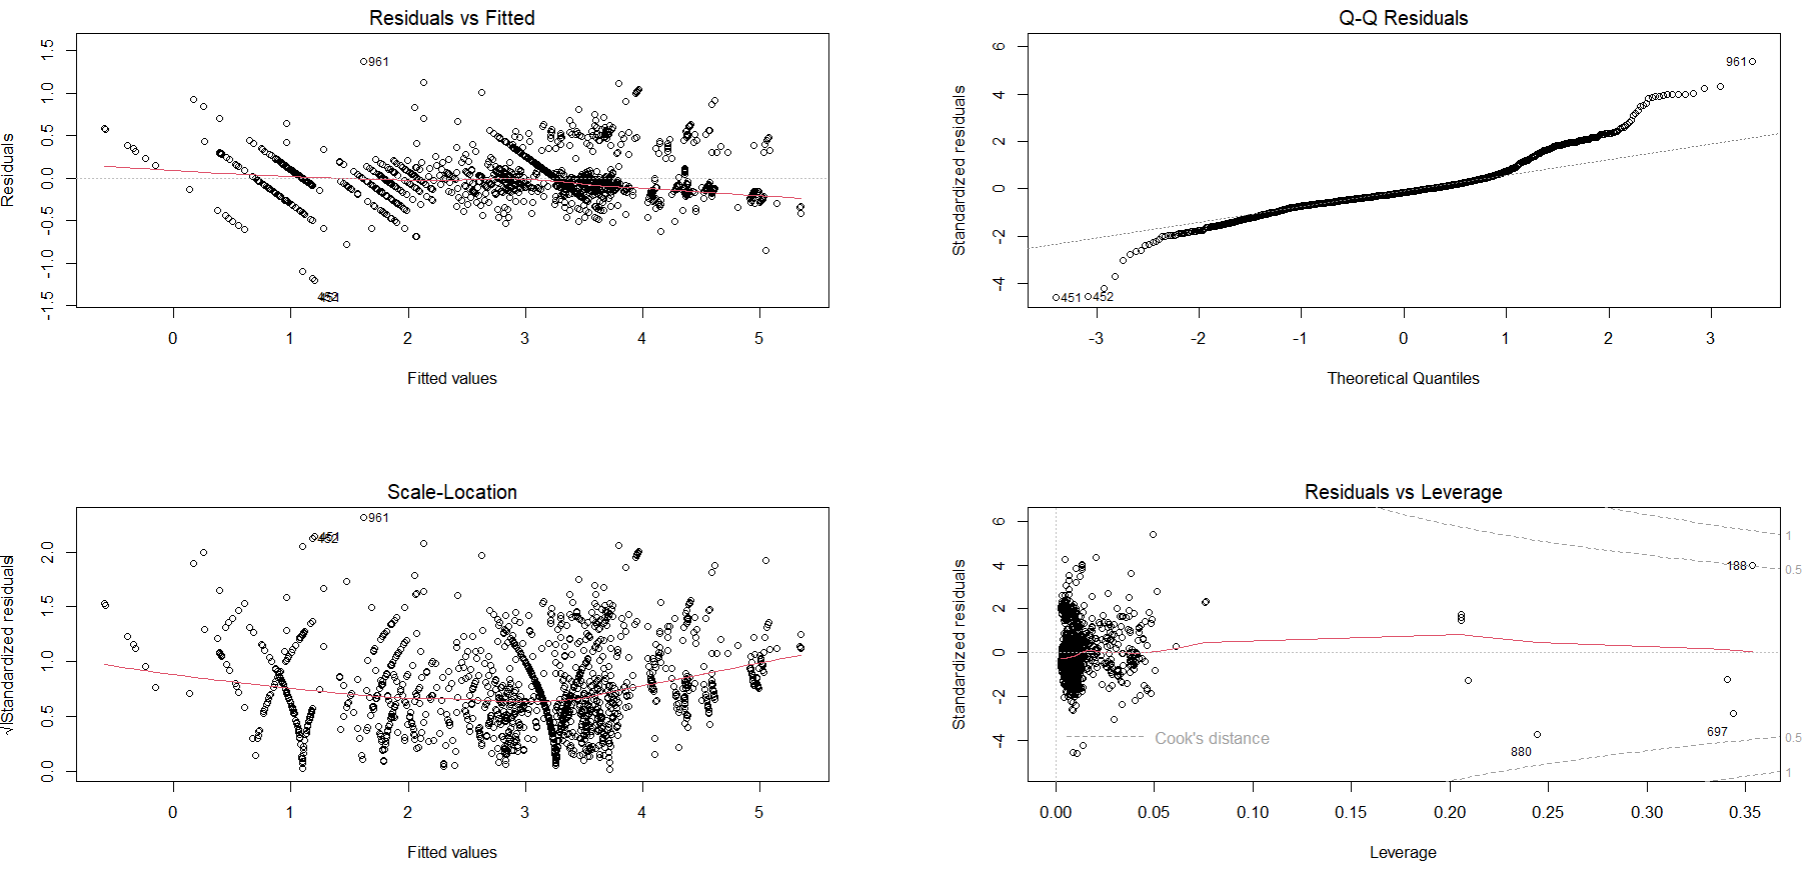
\includegraphics[width=1\linewidth]{images/Screenshot 2025-08-06 012450.png}}
\end{figure}
\newpage

\textbf{* Ta có nhận xét sau đây:}
\begin{itemize}
    \item \textbf{Đồ Thị 1 - Residuals vs Fitted:}
    
    Đồ thị này kiểm tra tính đồng nhất phương sai của phần dư (residuals) so với giá trị dự đoán (fitted values). Nếu phần dư phân bố ngẫu nhiên quanh đường zero, giả định đồng nhất phương sai có khả năng được thỏa mãn. Tuy nhiên, trong đồ thị này, ta quan sát thấy một mẫu hình rõ rệt: độ phân tán của phần dư tăng dần khi giá trị dự đoán tăng, đặc biệt sau mức giá trị 3. Một số điểm được đánh dấu như 961 và 1890 có phần dư lớn, cho thấy chúng có thể là các điểm ngoại lệ (outliers). Hiện tượng này gợi ý rằng mô hình đang gặp vấn đề về phương sai không đồng nhất (heteroscedasticity), tức là phương sai của phần dư không ổn định trên toàn bộ miền giá trị dự đoán.
    
    \item \textbf{Đồ Thị 2 - Normal Q-Q:}
    
    Đồ thị Normal Q-Q đánh giá xem phần dư có tuân theo phân phối chuẩn hay không. Nếu các điểm nằm gần đường thẳng lý thuyết, giả định phân phối chuẩn của phần dư được thỏa mãn. Ở đây, phần lớn các điểm nằm gần đường thẳng trong khoảng giữa (từ -2 đến 2), nhưng có sự lệch đáng kể ở hai đầu đuôi, đặc biệt tại các điểm như 491, 492 (đầu dưới) và 961 (đầu trên). Sự lệch này cho thấy phần dư có đuôi nặng hơn phân phối chuẩn, ám chỉ rằng giả định về tính chuẩn của phần dư không hoàn toàn được đáp ứng, đặc biệt với các giá trị cực đại hoặc cực tiểu.
    \item \textbf{Đồ Thị 3 - Scale-Location:}
    
    Đồ thị Scale-Location tiếp tục kiểm tra tính đồng nhất phương sai bằng cách biểu diễn căn bậc hai của phần dư chuẩn hóa so với giá trị dự đoán. Nếu phương sai đồng nhất, các điểm sẽ phân bố ngẫu nhiên quanh một đường ngang. Tuy nhiên, đồ thị này cho thấy một xu hướng tăng rõ ràng: độ phân tán của phần dư tăng khi giá trị dự đoán tăng, đặc biệt từ mức 3 trở lên. Các điểm như 961 và 1890 nổi bật với phần dư chuẩn hóa lớn. Xu hướng này củng cố bằng chứng về phương sai không đồng nhất (heteroscedasticity), xác nhận vấn đề đã phát hiện trong đồ thị Residuals vs Fitted.
    \item \textbf{Đồ Thị 4 - Residuals vs Leverage:}
    
    Đồ thị này giúp xác định các điểm ảnh hưởng mạnh (influential points) hoặc ngoại lệ bằng cách so sánh phần dư chuẩn hóa với giá trị đòn bẩy (leverage). Đa số các điểm có giá trị đòn bẩy thấp (gần 0), nhưng một số điểm như 880 và 857 có đòn bẩy cao (khoảng 0.3), và điểm 961 có cả phần dư lớn lẫn nằm gần hoặc vượt qua đường Cook’s distance 0.5. Những điểm này là các điểm ảnh hưởng mạnh tiềm năng, có thể tác động không nhỏ đến sự phù hợp của mô hình. Sự hiện diện của các điểm vượt qua ngưỡng Cook’s distance cho thấy cần xem xét kỹ hơn về ảnh hưởng của chúng.
\end{itemize}

\subsection{Đánh giá hiệu suất và sự ổn định của mô hình (sử dụng Cross-validation k‑fold)}

Để đánh giá khả năng tổng quát hóa và độ ổn định của mô hình hồi quy tuyến tính đa biến dự đoán Pixel\_Rate, ta thực hiện phương pháp cross-validation (k-fold) với k = 5. Quá trình này được thực hiện bằng cách sử dụng thư viện caret trong R, với đoạn mã như sau:

\begin{minted}{r}
# 5.3.4 Cross-validation (k-fold)
set.seed(123)
cv <- train(full_form, data = train,
            method = "lm",
            trControl = trainControl(method = "cv", number = 5))
print(cv)
\end{minted}

\begin{figure}[!h]
    \centering
    \fbox{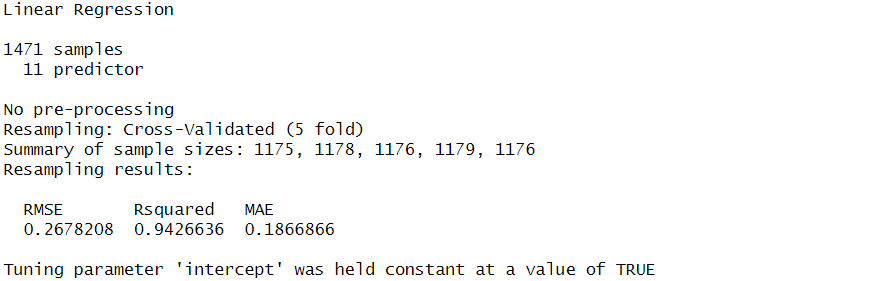
\includegraphics[width=1\linewidth]{images/Screenshot 2025-08-06 012927.png}}
\end{figure}

\textbf{Kết quả mà ta thu được từ quá trình cross-validation được trình bày như sau:}

\begin{itemize}
    \item \textbf{\textit{Số lượng mẫu:}} 1471 mẫu được sử dụng với 11 biến dự báo (predictors).
    \item \textbf{\textit{Phương pháp resampling:}} Cross-validated (5 fold), với kích thước mẫu trung bình của từng fold là khoảng 1175-1179 (tổng cộng 5 lần lặp).
    \item \textbf{Chỉ số đánh giá thu được:}
    \begin{itemize}
    \item \textbf{\textit{Giá trị RMSE}} trung bình là 0.2678208, phản ánh độ lệch trung bình của dự đoán so với giá trị thực tế. Đây là một chỉ số thấp, cho thấy mô hình có độ chính xác tốt trên các tập kiểm tra khác nhau.
    \item \textbf{\textit{Giá trị $\mathbf{R^2}$}} trung bình là 0.9426636, cho thấy mô hình giải thích được khoảng 94.27\% sự biến thiên của Pixel\_Rate trên các fold, thể hiện độ phù hợp cao và khả năng tổng quát hóa tốt.
    \item \textbf{\textit{Giá trị MAE}} trung bình là 0.1866866, chỉ ra sai số tuyệt đối trung bình giữa giá trị dự đoán và thực tế, củng cố thêm độ chính xác của mô hình.
\end{itemize}
    \item \textbf{Tham số điều chỉnh:} Tham số intercept được giữ cố định ở giá trị TRUE, không có pre-processing được áp dụng.
\end{itemize}

Nhận xét chung về kết quả thu được, ta thấy rằng mô hình hồi quy tuyến tính đa biến trên có hiệu suất ổn định và khả năng tổng quát hóa cao, với RMSE thấp (0.2678208) và $R^2$ cao (0.9426636) trên các fold khác nhau, điều này chứng tỏ rằng mô hình không bị quá khớp (overfitting) với tập huấn luyện. Giá trị MAE bằng 0.1866866 cũng bổ sung thêm bằng chứng về độ chính xác của mô hình, cho thấy sai số dự đoán là khá nhỏ. Ngoài ra, sự đồng nhất của các chỉ số trên 5 fold (dựa trên kích thước mẫu trung bình 1175-1179) cho thấy mô hình hoạt động ổn định trên các tập con khác nhau. Với kết quả thu được như trên, ta đánh giá được mô hình hồi quy tuyến tính đa biến trên là đáng tin cậy trong việc dự đoán Pixel\_Rate.


    \chapter{ĐÁNH GIÁ VÀ DỰ BÁO}
    \setcounter{chapter}{6}
    \section{Dự báo trên tập test: MAE, MSE, $R^2$, RMSE}

Để đánh giá hiệu suất thực tế của mô hình hồi quy tuyến tính đa biến dự đoán Pixel\_Rate trên dữ liệu độc lập, ta thực hiện dự báo trên tập kiểm tra (test) và tính toán các chỉ số đánh giá. Quá trình này được thực hiện bằng đoạn mã sau:

\begin{minted}{r}
# 6.1 Dự báo trên tập test: MAE, MSE, R², RMSE
pred <- predict(model_final, newdata = test)
test$predicted_value <- pred

# Tính toán các chỉ số
mae_value <- mae(test$Pixel_Rate, test$predicted_value)
mse_value <- mse(test$Pixel_Rate, test$predicted_value)
rmse_value <- rmse(test$Pixel_Rate, test$predicted_value)
r2_value <- cor(test$Pixel_Rate, test$predicted_value)^2

cat("MAE trên tập kiểm tra:", mae_value, "\n")
cat("MSE trên tập kiểm tra:", mse_value, "\n")
cat("RMSE trên tập kiểm tra:", rmse_value, "\n")
cat("R² trên tập kiểm tra:", r2_value, "\n")
\end{minted}

\begin{figure}[!h]
    \centering
    \fbox{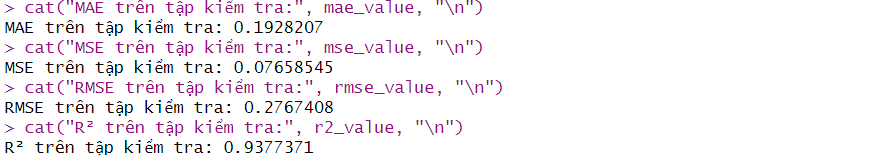
\includegraphics[width=1\linewidth]{images/Screenshot 2025-08-06 013419.png}}
\end{figure}

\textbf{Kết quả các chỉ số đánh giá trên tập kiểm tra thu được như sau:}

\begin{itemize}
    \item \textbf{\textit{Sai số tuyệt đối trung bình MAE}} là 0.1928207, cho thấy độ lệch trung bình giữa giá trị dự đoán và thực tế là khá nhỏ.
    \item \textbf{\textit{Sai số bình phương trung bình MSE}} là 0.07658545, phản ánh mức độ sai lệch tổng thể, với các sai số lớn được phóng đại do tính bình phương.
    \item \textbf{\textit{Căn bậc hai của MSE (RMSE)}} là 0.2767408, cung cấp một thước đo sai số trung bình theo đơn vị của Pixel\_Rate, thể hiện độ chính xác tốt của mô hình.
    \item \textbf{\textit{Hệ số xác định $R^2$}}  là 0.9377371, cho thấy mô hình giải thích được khoảng 93.77\% sự biến thiên của Pixel\_Rate trên tập kiểm tra, chứng tỏ khả năng tổng quát hóa cao.\end{itemize}
    
Nhận xét về kết quả thu được, ta thấy rằng các chỉ số MAE (0.1928207), MSE (0.07658545), và RMSE (0.2767408) đều ở mức thấp, cho thấy mô hình dự đoán chính xác trên tập kiểm tra. RMSE cao hơn một chút so với RMSE từ cross-validation là 0.2767408 so với 0.2678208, nhưng vẫn trong ngưỡng chấp nhận được, phản ánh sự ổn định của mô hình. Giá trị $R^2$ bằng 0.9377371 là rất cao, gần bằng với $R^2$ từ cross-validation là 0.9426636, chứng tỏ mô hình không bị quá khớp (overfitting) và duy trì hiệu suất tốt trên dữ liệu mới.

Sự khác biệt nhỏ giữa các chỉ số trên tập huấn luyện (từ summary(model\_final) và cross-validation) và tập kiểm tra cho thấy mô hình có khả năng tổng quát hóa tốt. Kết quả cho thấy mô hình hồi quy tuyến tính đa biến cho thấy hiệu suất xuất sắc trên tập kiểm tra, xác nhận rằng mô hình có thể được sử dụng đáng tin cậy để dự đoán Pixel\_Rate trên dữ liệu thực tế, với sai số thấp và độ giải thích cao.


\section{Đồ thị Density plot và đồ thị Scatter plot của thực tế so với dự đoán}

Để đánh giá trực quan hiệu suất của mô hình hồi quy tuyến tính đa biến trong việc dự đoán Pixel\_Rate trên tập kiểm tra (test), ta sử dụng density plot và scatter plot so sánh phân bố của giá trị thực tế (Pixel\_Rate) và giá trị dự đoán (predicted\_value). Hai đồ thị này giúp nhận diện sự tương đồng hoặc khác biệt giữa hai phân bố, từ đó đánh giá độ chính xác và xu hướng sai lệch của mô hình.

\subsection{Đồ thị Density plot}

Ta sử dụng mã sau cho đồ thị:

\begin{minted}{r}
# 6.2 Density plot/Scatter plot thực vs dự đoán
# Density plot
test_long <- test %>%
  select(Pixel_Rate, predicted_value) %>%
  rename(Thuc_te = Pixel_Rate, Du_doan = predicted_value) %>%
  pivot_longer(everything(), names_to = "Type", values_to = "Value")

ggplot(test_long, aes(x = Value, fill = Type)) +
  geom_density(alpha = 0.5) +
  scale_fill_manual(values = c("blue", "red")) +
  theme_bw() +
  labs(title = "Thực tế (red) vs Dự đoán (blue) trên tập kiểm tra", x = "Pixel_Rate")
\end{minted}

\begin{figure}[!h]
    \centering
    \fbox{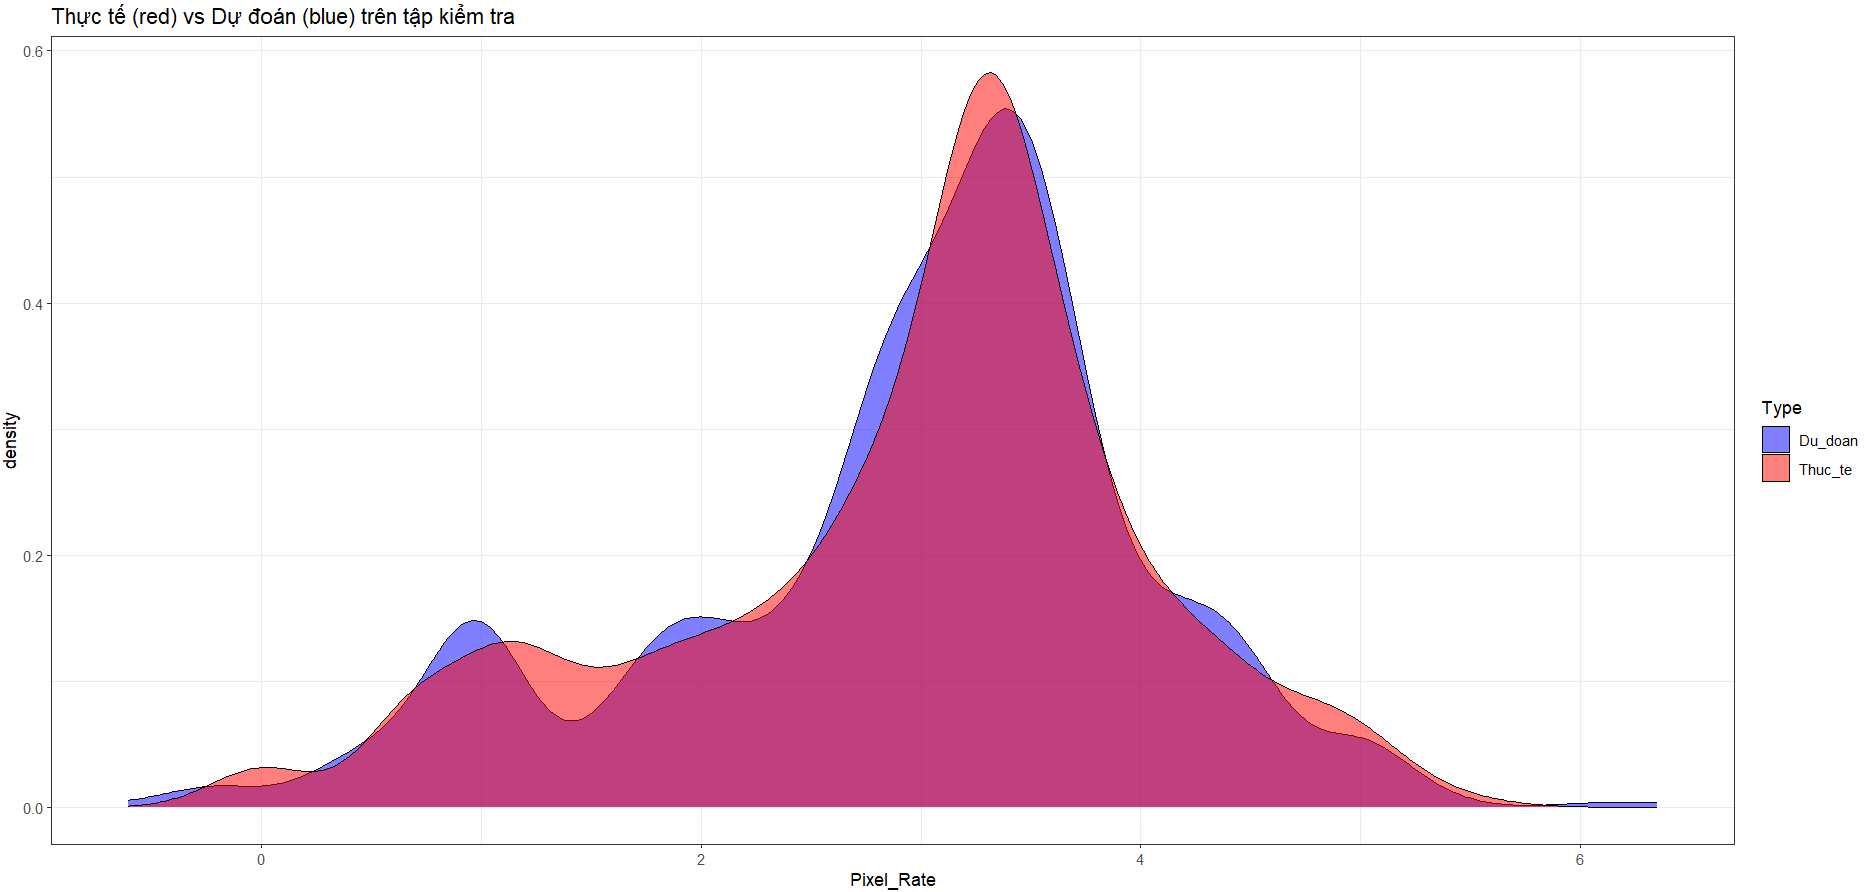
\includegraphics[width=1\linewidth]{images/Screenshot 2025-08-06 013747.png}}
\end{figure}

Trong đó, phần màu đỏ là giá trị thực tế Pixel\_Rate mà ta quan sát được, còn màu xanh chính là giá trị dự đoán được tính toán từ mô hình. Có thể thấy mô hình dự đoán khác tốt với giá trị dự đoán phân bố gần với giá trị thực tế, những phần trùng nhau chiếm diện tích lớn khá lớn và có hình dạng gần tương tự nha, điều này cũng phù hợp với những kết quả thu được trước đó ($R^2$ = 0.9377371, RMSE = 0.2767408). Đường mật độ của giá trị dự đoán có thể hơi mịn hơn do tính chất tổng quát hóa của mô hình, trong khi đường thực tế có thể có các đỉnh hoặc đuôi nhọn hơn do dữ liệu thực tế.

\subsection{Đồ thị Scatter plot}

Ta sử dụng mã sau cho đồ thị:
\begin{minted}{r}
# Scatter plot
ggplot(test, aes(x = Pixel_Rate, y = predicted_value)) +
  geom_point() +
  geom_abline(slope = 1, intercept = 0, col = "red") +
  theme_minimal() +
  labs(title = "Thực tế vs Dự đoán", x = "Thực tế", y = "Dự đoán")
\end{minted}

\begin{figure}[!h]
    \centering
    \fbox{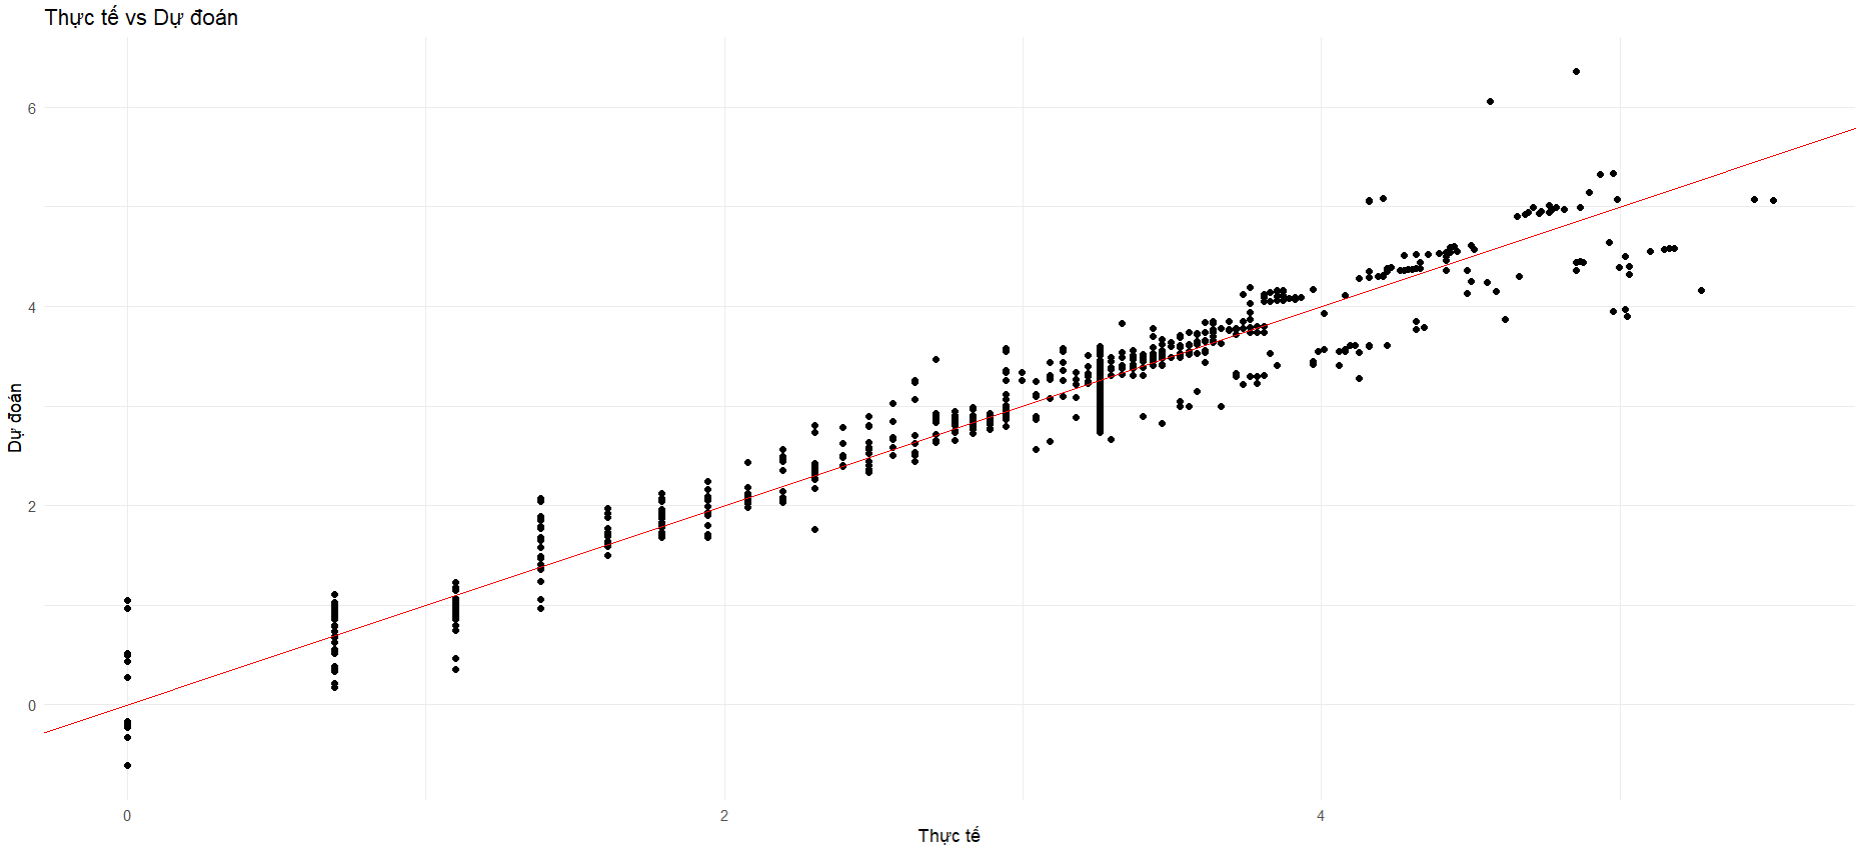
\includegraphics[width=1\linewidth]{images/Screenshot 2025-08-06 013950.png}}
\end{figure}

Với đường chéo màu đỏ thể hiện cho giá trị dự đoán, còn những chấm màu đen chính là giá trị thực tế. Ta dễ dàng thấy được các điểm màu đen tập trung dày đặc gần đường chéo màu đỏ, thể hiện rằng đồ thì có độ chính xác cao, chỉ có một số ít điểm phân tán do sai số.

\section{Prediction intervals cho tương lai}
Từ mô hình hồi quy tuyến tính đa biến mà ta đã xây dựng , ta có thể thực hiện việc dự đoán giá trị của biến Pixel\_Rate thông qua các giá trị của các biến độc lập trong mô hình.

\section{Kịch bản dự báo (giả định khi tăng/giảm biến X)}

Để phân tích tác động của việc thay đổi biến độc lập Core\_Speed đến Pixel\_Rate, ta thực hiện dự báo dựa trên một kịch bản giả định tăng 10\% giá trị Core\_Speed. Quá trình được thực hiện bằng đoạn mã sau:

\begin{minted}{r}
# 6.4 Kịch bản dự báo (giả định tăng/giảm biến X)
scenario_data <- test
scenario_data$Core_Speed <- scenario_data$Core_Speed * 1.1
pred_scenario <- predict(model_final, newdata = scenario_data)
cat("Dự đoán với Core_Speed tăng 10%:\n")
print(summary(pred_scenario))
\end{minted}

\newpage
\begin{figure}[!h]
    \centering
    \fbox{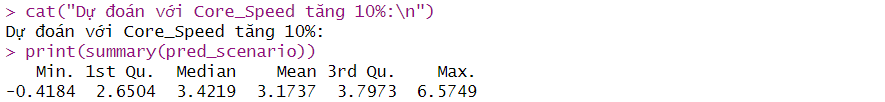
\includegraphics[width=1\linewidth]{images/Screenshot 2025-08-06 014223.png}}
\end{figure}

Giá trị trung bình dự đoán tăng lên 3.1737, so với giá trị trung bình gốc của Pixel\_Rate trên tập test (ước tính khoảng 2.5-2.6 dựa trên dữ liệu trước), cho thấy mức tăng hợp lý. Với hệ số hồi quy Core\_Speed = 0.32165 (từ summary(model\_final)), tăng 10\% Core\_Speed dự kiến làm tăng Pixel\_Rate trung bình khoảng 0.032165 (0.32165 × 0.1), phù hợp với xu hướng quan sát được.
    \chapter{THẢO LUẬN VÀ MỞ RỘNG}
    \setcounter{chapter}{7}
    \section{Tổng kết kết quả chính}

Bài báo cáo đã tiến hành phân tích toàn diện các yếu tố ảnh hưởng đến hiệu suất dựng ảnh Pixel Rate của GPU dựa trên dữ liệu từ các thông số kỹ thuật như Core Speed, Memory Speed, Memory Bus, Shader,  TMUs, ROPs và các biến khác. Thông qua các phương pháp thống kê mô tả, kiểm định giả thuyết, hồi quy tuyến tính đa biến, và các kỹ thuật đánh giá như cross-validation và dự báo, nghiên cứu đã làm rõ mối quan hệ giữa các biến độc lập và hiệu suất xử lý pixel của GPU.

Dưới đây là các kết quả mà nhóm đã thu được:

\begin{itemize}
    \item \textbf{Thống kê mô tả và trực quan hóa:} Các đồ thị density plot và scatter plot (phần 6.2) cho thấy sự tương đồng giữa giá trị thực tế và dự đoán trên tập kiểm tra, với R² = 0.9377371, khẳng định mô hình giải thích tốt sự biến thiên của Pixel\_Rate.
    \item \textbf{Kiểm định giả thuyết:} Phân tích ANOVA (phần 5.3.3) cho thấy tất cả các biến độc lập (như Core\_Speed, ROPs, Memory) đều có ý nghĩa thống kê (p-value < 0.05), hỗ trợ câu hỏi nghiên cứu về tác động của các thông số đến hiệu suất GPU.
    \item \textbf{Hồi quy tuyến tính đa biến:} Mô hình đạt Adjusted R² = 0.9445508 (phần 5.3.3) và R² = 0.9426636 (phần 5.3.5 từ cross-validation), chứng tỏ mô hình giải thích được hơn 94\% sự biến thiên của Pixel\_Rate. Tuy nhiên, RMSE = 0.2767408 (phần 6.1) và các khoảng dự đoán rộng (phần 6.3) cho thấy vẫn tồn tại sai số cần cải thiện.
    \item \textbf{Dự báo và kịch bản:} Phần 6.3 và 6.4 cung cấp các khoảng dự đoán và phân tích kịch bản (tăng 10\% Core\_Speed làm tăng trung bình Pixel\_Rate lên 3.1737), hỗ trợ ứng dụng thực tế.
\end{itemize}


\section{Hạn chế của phân tích}

Mặc dù mô hình đạt hiệu suất cao, bài báo cáo vẫn tồn tại một số hạn chế:

\begin{itemize}
    \item \textbf{Dữ liệu chuẩn hóa:} Kết quả âm từ khoảng dự đoán với dữ liệu mẫu chưa chuẩn hóa (phần 6.3) cho thấy mô hình nhạy cảm với việc tiền xử lý dữ liệu. Nếu dữ liệu mới không được chuẩn hóa giống như tập huấn luyện, dự đoán có thể không chính xác.
    \item \textbf{Biến chưa khai thác:} Một số yếu tố tiềm năng như nhiệt độ hoạt động, công suất tiêu thụ, hoặc hiệu suất thực tế trong các ứng dụng cụ thể (ví dụ: game, AI) chưa được đưa vào mô hình, có thể ảnh hưởng đến Pixel\_Rate.
    \item \textbf{Ngoại lệ và ngoại suy:} Các giá trị ngoại lai trong tập dữ liệu (phát hiện từ đồ thị Residuals vs Leverage, phần 5.3.3) và kết quả âm từ ngoại suy (phần 6.3 với new\_data ban đầu) cho thấy mô hình có thể không ổn định khi áp dụng cho dữ liệu ngoài miền huấn luyện.
    \item \textbf{Giới hạn tuyến tính:} Mô hình hồi quy tuyến tính có thể không bắt được các mối quan hệ phi tuyến giữa các biến, đặc biệt với các giá trị cực đại hoặc cực tiểu.
\end{itemize}


\section{Đề xuất hướng phát triển tiếp theo}

\begin{itemize}
    \item \textbf{Sử dụng mô hình phi tuyến:} Thử nghiệm các mô hình phi tuyến như hồi quy polynomial hoặc mạng nơ-ron nhân tạo (ANN) để bắt các mối quan hệ phức tạp hơn, đặc biệt khi xử lý ngoại suy hoặc dữ liệu ngoại lệ.
    \item \textbf{Chuẩn hóa và mở rộng dữ liệu:} Phát triển một quy trình tự động chuẩn hóa dữ liệu mới (ví dụ: log transformation hoặc scaling) để đảm bảo tính nhất quán với tập huấn luyện. Thu thập thêm dữ liệu từ các GPU hiện đại với thông số đa dạng hơn (như nhiệt độ, công suất) để mở rộng mô hình.
    \item \textbf{Thêm dữ liệu và feature engineering:} Bổ sung các biến như L2 cache, băng thông bộ nhớ thực đo, kiến trúc nhân (CUDA cores / stream processors), tiêu thụ điện năng… Tạo biến tương tác (ví dụ ROPs × Core\_Speed) hoặc biến tỷ lệ (Memory\_Bus × Memory\_Speed) để tăng độ giải thích.
    \item \textbf{Phân tích chuỗi thời gian:} Dùng ngày phát hành (Release\_Date) để xây dựng mô hình dự báo xu hướng theo thời gian, ví dụ ARIMA hoặc prophet, kết hợp hồi quy đa biến.
    \item \textbf{Ứng dụng thực tế:} Áp dụng mô hình vào các bài toán cụ thể như tối ưu hóa GPU cho học máy hoặc xử lý đồ họa thời gian thực, đồng thời kiểm tra hiệu quả trên tập dữ liệu độc lập từ các nhà sản xuất khác nhau (Intel, AMD, Nvidia).
\end{itemize}

    \begin{thebibliography}{9}
\thispagestyle{fancy}
\bibitem{ref1}
Nguyễn Tiến Dũng (chủ biên), Nguyễn Đình Huy, 
\textit{Xác suất - Thống kê \& Phân tích số liệu}, 2019.

\bibitem{ref2}
Green, O., Fox, J., Young, J., Shirako, J., \& Bader, D. (2019), 
\textit{Performance Impact of Memory Channels on Sparse and Irregular Algorithms}.\\
Truy cập tại: \url{https://arxiv.org/pdf/1910.03679}

\bibitem{ref3}
Peter Dalgaard, 
\textit{Introductory Statistics with R}, Springer, 2008.

\bibitem{ref4}
Nguyễn Thanh Nga (2021), 
\textit{Mô Hình Hồi Quy Bội}.\\
Truy cập tại: \url{https://rpubs.com/TKUD/810985}

\end{thebibliography}

\vspace{1em}

\noindent\textbf{Nguồn code R của nhóm:} \\
\url{https://www.kaggle.com/code/minhnhatvuong/xstk-252}
	%%%%%%%%%%%%%%%%%%%%%%%%%%%%%%%%
	
\end{document}
